\documentclass{cslthse-msc}
\usepackage[T1]{fontenc}
\usepackage[utf8x]{inputenc}
\usepackage[english]{babel}
\usepackage{amsmath}
\usepackage{amsfonts}
\usepackage{amssymb}
\usepackage{amsthm}
\usepackage{breqn}
%\usepackage{makeidx}
\usepackage{graphicx}
\usepackage{framed}
\usepackage{tikz}
\usetikzlibrary{calc, shapes, backgrounds, positioning, matrix, shapes.multipart}
\usepackage{standalone}
\usepackage[titletoc, header, page]{appendix}
\usepackage{pdflscape}
\usepackage{hyperref}
\usepackage{mdwlist}
\usepackage{multirow}
\usepackage{float}
\usepackage{pgfplots}
\usepackage{listings}

%\geometry{showframe}

\author{
	Tommy Kvant \\
	{\normalsize \href{mailto:ada09tkv@student.lu.se}{\texttt{ada09tkv@student.lu.se}}}
}

\title{Task scheduling for dual-arm industrial robots through constraint programming\\\large MiniZinc modeling and solver comparison}

\supervisor{Jacek Malec, \href{mailto:jacek.malek@cs.lth.se}{\texttt{jacek.malek@cs.lth.se}}}
\assSupervisor{Maj Stenmark, \href{mailto:maj.stenmark@cs.lth.se}{\texttt{maj.stenmark@cs.lth.se}}}
%\supervisor{Maj Stenmark, \href{mailto:maj.stenmark@cs.lth.se}{\texttt{maj.stenmark@cs.lth.se}}}
\examiner{Klas Nilsson, \href{mailto:klas.nilsson@cs.lth.se}{\texttt{klas.nilsson@cs.lth.se}}}

\acknowledgements{

}

\theabstract{

}

\keywords{key word}

\begin{document}
\makefrontmatter
\chapter{Introduction} 

More and more of the production in today's society is getting automated. Manufacturers want to cut cost and make the production more effective by eliminating the human work and replace it with robots. But there are drawbacks; robots are expensive and robots does not have the versatility of a human. This puts pressure on the robot manufacturers to develop robots that are more versatile. Thus eliminating the need to have multiple robots to do multiple tasks which will lower the costs and also making the robots more versatile, closing the gap of what a human and robots are able to do.

Current robot setups usually have one robot performing one task all the time, as opposed to flexible robots which will be performing many different tasks and assemblies. One of these robots is ABB's robot YuMi\textsuperscript\textregistered. YuMi\textsuperscript\textregistered is a dual armed robot made to work alongside humans and able to perform some of the most complex tasks, such as mount a nut or thread a needle\cite{_yumi_}. It accomplishes this by using a wide variety of sensors, e.g., force sensor, visual sensors, etc. Usually a robot replaces humans to perform dangerous or heavy tasks, while YuMi\textsuperscript\textregistered is mainly designed for small parts cooperation with humans, i.e. usually human roles in todays manufacturing environment.

Flexible robots such as YuMi\textsuperscript\textregistered poses the demand for the scheduling of such robots to be flexible as well. A scheduling of a robot can be a time consuming task. Since manufacturers want as effective assemblies as possible, it can take from days to weeks to perfect an assembly schedule. This is not feasible if you want to use the robot for many different tasks and assemblies. In this thesis we would like to try and automate this scheduling process in order to cut down on the scheduling time. To accomplish this we will be using Constraint programming, as it provides a general interface to solve problems without needing to build a complete framework from scratch. Also, scheduling is a classical constraint problem, thus constraint programming suits this problem well.





\section{Project goal}
The goal of this thesis is to present a generic CP model suitable for a robot such as YuMi\textsuperscript\textregistered, able to handle the type of jobs YuMi\textsuperscript\textregistered is able to perform. It will be constructed using the MiniZinc language and tested using 6 CP solvers. We will compare the results the results from the solvers, both to see how well our model can perform and how well the solvers perform relative to one another.

\section{Related work}
\cite{sethi_2006} conclude that the increasing number of machines in a robotic cell causes an explosive growth in combinatorial possibilites. They also provide evidence that a dual-gripper cell is more productive than a single-gripper cell.

\cite{thornblad_2013} concludes that when a cell is part of an assembly flow, the targeting of due dates instead of makespan is to prefer. The reason is that the focusing on makespan runs the risk of exacerbating an already unreliable flow. However, the assembly we want to construct is not a part of a flow, and thus we do not concern ourselves with maintaining a stable flow through the cell, but only to optimize the assembly in the cell.

\cite{yuan_2013} states that constraint programming is only effective on small problems of flexible job shop scheduling. In order to effectively solve problems of larger size they suggest to use methods such as large neighbourhood search (LNS) or iterative flattening search. They also show that LNS together with Hybrid Harmonic Search produces good results.
\\
Unfortunately MiniZinc does not support the implementation of custom searches such as LNS. Therefore we try to solve the problem of ineffectiveness by using filter such as those presented by Vilím in \cite{VilimBartak2002Batch} \cite{Vilim2002Precedence} and \\\cite{VilimBartak2002Sequence}.

\cite{ejenstam_2014} conducted a similar study also on the YuMi\textsuperscript\textregistered robot. In the study Google or-tools was used to write the model and also implemented \emph{Systematic Tree Search}, \emph{Random Restart} and \emph{Local Search} and compared the results of using different combinations of them. The case study and goal of the study is different from this thesis and therefore the resulting models differ, as is discussed in chapter \ref{cha:discuss}. In the study it was conclude that \emph{Systematic Tree Search} combined with \emph{Random Restart} produced schedules with better results than the reference solution.
\\\\
Unfortunately, not many comparisons between MiniZinc solvers where found. There is an annual competition held by NICTA where solvers can compete, this is the most comprehensive documentation of the performance of the solvers we have found. Unfortunately, they only present which solver wins a category and no statistics are presented. Hence, no deeper comparison can be made from the result. In the latest competition held, 2014, or-tools won three out of the four gold medals, Opturion CPX won all four silver medals and Choco won three out of the four bronze medals\cite{mz_result_2014}.

When presenting MiniZinc for the first time, initial tests were also presented comparing, amongst others, G12/FD, Gecode using FlatZinc code and native Gecode. The tests show that MiniZinc was competitive with the native Gecode model and on average the Gecode front-end for FlatZinc was about 200ms faster than the G12/FD\cite{mz_paper}.

Another comparison found was \cite{nicta_2964} where they tested 10 solver on 12 problems. Unfortunately, the only solver tested there that we also used in this thesis is the G12/FD solver. So comparison with our results is hard. Although they did not draw any conclusions, G12/FD seem to fare relatively well compared to the other solvers tested.


\section{Report structure}
First we will present the approach we have taken in the thesis and present the relevant background information in chapter \ref{cha:approach}. In chapter \ref{cha:assembly} we will present the case study assembly used in the thesis. Then we will present an in depth view of the model created in chapter \ref{cha:model}.  In chapter \ref{cha:eval} we will present the setup used to evaluate the model and the result of the evaluation. In chapter \ref{cha:discuss} we will discuss the results and we will come to a conclusion in chapter \ref{cha:conc}.
\\\\
Lastly we have two appendices. Appendix \ref{app:ext_mod} contains parts of the model which is not crucial for solving of the problem, but is still a part of the model. In appendix \ref{app:tool_manuals} we present all the tools used, which are free for anyone to use, and where to acquire them.

\chapter{Approach}\label{cha:approach}

\section{Constraint Programming}
Constraint programing is a \emph{declarative} paradigm. This means that in contrast to \emph{imperative} paradigm languages, such as C or Java, the focus of solving problems using constraint programming is on specifying the problem and not the algorithm to solve it. However, \emph{declarative} languages, such as Java and C, can be used as a framework Constraint Programming, as in JaCoP, or-tools, and others. One specifies the \emph{domain variables}, or simply variables, and \emph{constraints}. Variables have domains of values, meaning they can take any value in their domain. Variables can often be, depending on language and solver, either integers, floating-points, boolean or symbolic, symbolic being a text or label. For example a symbolic variable representing a week would have the domain\\
$\{Monday,Tuesday, Wednesday, Thursday, Friday, Saturday, Sunday\}$, while an integer one could have $\{0,1,2,3,4,5,6\}$.

\subsection{Constraints}
Constraints are set up as relationships between the variables, and thereby limiting the domains of the variables. Integer domains are often used for variables, so for the rest of this section we will assume variables have integer domains. For this domain the following function symbols can be used: $+$, $\times$, $-$ and $\div$. The constraint relation symbols are $=$, $<$, $\leq$, $>$, $\geq$, $\neq$. Together with the function symbols and the constraint relation symbols, one can create simple constraint, called \emph{primitive constraint}. An example of a primitive constraint is $X < Y$, i.e.\ the values in $X$'s domain has to be lower than in $Y$'s. Primitive constraints can be used to create more complex constraints using the conjunctive connective $\land$. An example of this is $X < Y \land Y < 10$, i.e.\ $Y$ has to be less than $10$ and $X$ has to be less than $Y$. Since all constraints have to hold when the model is evaluated, all constraints are implicitly joined by a conjunction. The disjunctive connective $\lor$ is also available and can be used in the same way as $\land$. 

For example, lets assume we have a problem with two variables, $X$ and $Y$, $X = 4$ and $Y = \{1..10\}$. Here $X$ has the value $4$ and can thereby only take the value $4$. $Y$ on the other hand can take the values $1$ to $10$. This means a solution to this problem can be $X = 4$ and $Y = 1$ or likewise $X = 4$ and $Y = 5$ , they are equally correct.\\
On this problem we can impose a constraint, for example $Y > X$. Now we have set the constraint that $Y$ needs to be larger than $X$. And since $X$ has a fixed known value we can directly see that $Y > 4$, since $x = 4$. Now with this constraint, we can reduce the domain of $Y$ and now $Y = \{5..10\}$ instead. And now a viable solution can be $X = 4$ and $Y = 7$, but not $X = 4$ and $Y = 3$.

\begin{figure}
  \documentclass{standalone}
\usepackage{tikz}
\usetikzlibrary{calc, shapes, backgrounds}
\usepackage{standalone}
\usepackage{amsmath, amssymb}
\pagecolor{olive!50!yellow!50!white}
\begin{document}
\tikzset{
  leaf/.style = {draw=none,label = center:\textsf{$\vdots$}},
  labels/.style={midway, sloped, above, yshift=-10pt}
}
\begin{tikzpicture}
[
    scale = 0.75, transform shape, thick,
    every node/.style = {draw, circle, minimum size = 5mm, line width = 1pt, align=center},
    grow = down,  % alignment of characters
    level 1/.style = {sibling distance=6cm},
    level 2/.style = {sibling distance=2cm}, 
    level 3/.style = {sibling distance=1cm}, 
    level distance = 3 cm
  ]
 \node (Start){}
   child {   node [] (A) {}
     child { node [] (D) {}
       child { node [leaf] (M) {}}
       child { node [leaf] (N) {}}
     }
     child { node [] (E) {}
       child { node [leaf] (O) {}}
       child { node [leaf] (P) {}}
     }
     child { node [] (F) {}
       child { node [leaf] (Q) {}}
       child { node [leaf] (R) {}}
     }
   }
   child {   node [] (B) {}
     child { node [] (G) {}
       child { node [leaf] (S) {}}
       child { node [leaf] (T) {}}
     }
     child { node [] (H) {}
       child { node [leaf] (U) {}}
       child { node [leaf] (V) {}}
     }
     child { node [] (I) {}
       child { node [leaf] (X) {}}
       child { node [leaf] (Y) {}}
     }
   }
   child{ node(C){}
     child { node [] (J) {}
       child { node [leaf] (Z) {}}
       child { node [leaf] (A1) {}}
     }
     child { node [] (K) {}
       child { node [leaf] (B1) {}}
       child { node [leaf] (C1) {}}
     }
     child { node [] (L) {}
       child { node [leaf] (D1) {}}
       child { node [leaf] (E1) {}}
     }
   };

  
  % Labels
  \begin{scope}[nodes = {draw = none}]
    \path (Start) -- (A) node [labels] {Pick $X$};
    \path (Start) -- (B) node [labels] {Pick $Y$};
    \path (Start) -- (C) node [labels] {Pick $Z$};
    \path (A)     -- (D) node [labels] {$X=1$};
    \path (A)     -- (E) node [labels] {$X=3$};
    \path (A)     -- (F) node [labels] {$X=6$};
    \path (B)     -- (G) node [labels] {$Y=5$};
    \path (B)     -- (H) node [labels] {$Y=9$};
    \path (B)     -- (I) node [labels] {$Y=8$};
    \path (C)     -- (J) node [labels] {$Z=6$};
    \path (C)     -- (K) node [labels] {$Z=3$};
    \path (C)     -- (L) node [labels] {$Z=5$};
    \path (D)     -- (M) node [labels] {Pick $Y$};
    \path (D)     -- (N) node [labels] {Pick $Z$};
    \path (E)     -- (O) node [labels] {Pick $Y$};
    \path (E)     -- (P) node [labels] {Pick $Z$};
    \path (F)     -- (Q) node [labels] {Pick $Y$};
    \path (F)     -- (R) node [labels] {Pick $Z$};
    \path (G)     -- (S) node [labels] {Pick $X$};
    \path (G)     -- (T) node [labels] {Pick $Z$};
    \path (H)     -- (U) node [labels] {Pick $X$};
    \path (H)     -- (V) node [labels] {Pick $Z$};
    \path (I)     -- (X) node [labels] {Pick $X$};
    \path (I)     -- (Y) node [labels] {Pick $Z$};
    \path (J)     -- (Z) node [labels] {Pick $X$};
    \path (J)     -- (A1) node [labels] {Pick $Y$};
    \path (K)     -- (B1) node [labels] {Pick $X$};
    \path (K)     -- (C1) node [labels] {Pick $Y$};
    \path (L)     -- (D1) node [labels] {Pick $X$};
    \path (L)     -- (E1) node [labels] {Pick $Y$};   
  \end{scope}
\end{tikzpicture}
\end{document} 
%     without .tex extension
  % or use \input{mytikz}
  \caption{The beginning of the search space for the variables $X$, $Y$, $Z$, where $X=\{1,3,6\}$ $Y=\{5,9,8\}$ $Z=\{6,3,5\}$}
  \label{fig:search_space}
\end{figure}

\subsection{Global constraints}
Global constraints are constraints that sets up a relation between an non-fixed number of variables and the global constraints can be reduced to a set of simpler binary constraints\\\cite{global_const}. They are also context independent\cite{global_constraint_catalogue}, which makes them quite convenient to use when modeling and we are using a couple of global constraints that are listed below.

The description of the global constraints in this section come from MiniZinc:s global constraints listing \cite{mz_global_constraints} and MiniZinc:s tutorial, \cite{mz_tute}.

\subsubsection{All Different Constraint (\texttt{allDifferent})}
The \texttt{allDifferent} constraint is pretty straightforward. It takes a set or an array \texttt{x} as argument and enforces all variables in \texttt{x} to take distinctly different values, i.e. all values will be different.

\subsubsection{Circuit Constraint (\texttt{circuit})}
The \texttt{circuit} constraint takes an array of integers representing  nodes, \texttt{x}. Each index is representing a node and the index is the number of the node. The value at the index represents the successor of the node at the index. \texttt{circuit} enforces the nodes to form a \emph{Hamiltonian circuit}. This means all nodes will be part of the circuit that is formed and no node will have itself as successor. See Figure \ref{fig:circuit} for an example.

\begin{figure}
\centering
\documentclass[border=4pt]{standalone}
\begin{document}

\sffamily
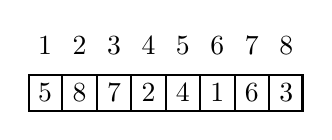
\begin{tikzpicture}[
  thick,
  myrect/.style={
    draw,
    rectangle split,
    rectangle split horizontal,
    rectangle split parts=#1,
    rectangle split part align=center
    } 
]

\node[myrect=8, draw=none](index)
  {
  \nodepart{one}1
  \nodepart{two}2
  \nodepart{three}3
  \nodepart{four}4
  \nodepart{five}5
  \nodepart{six}6
  \nodepart{seven}7
  \nodepart{eight}8
  };

\node[myrect=8, below of=index, yshift=0.4cm]
  {
  \nodepart{one}5
  \nodepart{two}8
  \nodepart{three}7
  \nodepart{four}2
  \nodepart{five}4
  \nodepart{six}1
  \nodepart{seven}6
  \nodepart{eight}3
  };

\end{tikzpicture}
\end{document}
\documentclass[border=4pt]{standalone}
\usetikzlibrary{arrows}
\begin{document}

\sffamily
\tikzstyle{arrow} = [thick,->,>=stealth]
\begin{tikzpicture}[node distance=1.5cm,
  thick
]

\node[draw, circle](1){1};
\node[draw, circle, right of=1](5){5};
\node[draw, circle, right of=5](4){4};
\node[draw, circle, right of=4](2){2};
\node[draw, circle, right of=2](8){8};
\node[draw, circle, right of=8](3){3};
\node[draw, circle, right of=3](7){7};
\node[draw, circle, right of=7](6){6}
	edge[arrow, bend left] (1);

\draw[arrow](1) -- (5);
\draw[arrow](5) -- (4);
\draw[arrow](4) -- (2);
\draw[arrow](2) -- (8);
\draw[arrow](8) -- (3);
\draw[arrow](3) -- (7);
\draw[arrow](7) -- (6);

\end{tikzpicture}
\end{document}
\caption{Example of the \texttt{circuit} constraint enforced on an array of length 8. The visualisation of the array on top. The visualisation of the nodes beneath with arrows from the node to its successor}
\label{fig:circuit}
\end{figure}

\subsubsection{Cumulative Constraint (\texttt{cumulative})}
The \texttt{cumulative} constraint is used to schedule entities that takes a given amount of resources in a system with a known amount of resources available. The constraint takes 5 arguments; an array of start times, an array of durations, an array of resources needed and an integer for how many resources available. So if we have $5$ resources available and we have two tasks which requires $3$ and $2$ resources respectively, they can execute simultaneously. But not if the number of available resources were $3$. Each index in the arrays corresponds to an entity.

\subsubsection{Global Cardinality constraint (\texttt{global\_cardinality})}
The \texttt{global\_cardinality} constraint takes three arguments; an array of variables \texttt{x}, an array of integer \texttt{cover}, and an array of variables \texttt{counts}. The constraint assures that the occurrences of \texttt{cover(i)} in \texttt{x} is equal to \texttt{counts(i)}.

\newpage

\subsection{Solver}
A Constraint Programming program consists of many of these constraints and variables. When the problem is specified in a model, a \emph{solver} runs the model. The goal of the solver is to satisfy all the constraints, i.e. set the domains of the variables so that they all follow the relationships of the constraints. This is called the \emph{constraint satisfaction problem}, and can  be defined as a triple $\langle Z,D,C \rangle$. $Z=\{x_1 \ldots x_n\}$ is a finite set of all the variables in the solution, $D(x_i), \; x_i \in Z$ is a set representing the domain of values the variable $x_i$ can assume, $C$ is the set of constraints imposed on the variables in $Z$. In order to satisfy all constraints imposed, the solver performs a \emph{search} on the space of possibilities, i.e.\ the \emph{search space}. The search space has the form of a tree, where each branch is a selection of a variable where the variables domain is reduced into a smaller subset that conforms with the constraints. The solver traverses the tree in search for a solution. When all variables are set to conform with the constraints a solution is found. If the solver reaches a node where a variable domain becomes empty, it has to \emph{backtrack} to a previous node from which it can choose a new variable to set, i.e.\ traversing a new branch of that node. To make sure that all constraints holds true, called \emph{consistency}, when a change occurs in a variable during search or by propagation itself, the solver performs \emph{propagation}. When a change occurs to a variable, lets call it $X$, the solver looks at the variables related to this variable through constraints, lets call them $Y$ and $Z$, and may prune the domains of $Y$ and $Z$ in order to uphold the consistency of the constraints. The solver then propagates onward to the variables related to $Y$ and $Z$ and performs the same procedure. More about solvers can be found in \cite{tsang_1993}, \cite{marriott_1998} and \cite{mz_manual}.

\subsection{Reified Constraints}
Reified constraints are constraints that couple a primitive constraint with a boolean variable and provide a relationship between the both. An example could be the constraint $c$ and a boolean variable $B$, the relationship between the both could be $c \Leftrightarrow B$. This says that if $c$ holds, $B = true$ and if $\neg c$ holds, $B = false$. This form of expression can be very useful in expressing complex relations and constraints \cite{marriott_1998}.

Although it is a convenient way of expressing complex relations, it has its disadvantages. Reified constraints can be inefficient since every reified constraint needs to be propagated all the time. Reified constraints can also propagate poorly, for example if a variable occurs multiple times in an expression \cite{jefferson_2010}. Due to this, we have tried to avoid direct reified constraints in the MiniZinc code in hope of reducing the total amount of reified constraints in the resulting code.

\subsection{Branching Heuristics}
Branching heuristics is what decides what value in a domain to branch on. It can be declared by the one programming the model and can play a significant role in the effectiveness of the model. An example of a common branching heuristic is \texttt{indomain\_min} which branches on the smallest value in the domain and if backtracked choses the next smallest value the next time, i.e.\ working its way up from the smallest value. The opposite of \texttt{indomain\_min} is \texttt{indomain\_max}, which starts in the other end of the domain. Another common branching heuristic is \texttt{indomain\_median} which branches on the median value of the domain and if backtracked branches on the values on either side of the median and works its way outwards. There are more branching heuristics available and which branching heuristics are available depend on the solver.

\section{Job-shop scheduling problem}
The job shop problem can be described as $n$ jobs of varying size containing a number of operations to be executed in a certain order that needs to be scheduled on $m$ identical machines. Commonly the goal is to minimize the total time for the schedule, called the \emph{makespan}. The traveling salesman problem is a version of the job shop problem where $m = 1$. \cite{garey_1976} shows that the job shop problem is NP-complete for $m \geq 2$ and $n \geq 3$, hence more complex versions of the job shop problem will be at least this hard.

As described above, the schedule is composed of jobs containing operations. This is the usual way of describing it in the literature, but we will look at it in a slightly different way. Instead of looking at many jobs, we will focus on one job and the operations within that job. In this thesis we will refer to these operations as tasks.
\\\\
An extension of the job shop problem is the flexible job shop problem. In it, tasks are not locked to be scheduled on a particular machine, but can be scheduled for any of the machines \cite{thornblad_2013}. This increases the complexity of the problem.
\\\\
Yet another extension of the job shop problem is the job shop problem with sequence-dependent setups. This means the time for a task is not just the time it takes to execute the task itself, but also the time it takes to set up the machine, depending on the previous task, in order to execute the task at hand. This is also something that increases the complexity compared to the basic job shop problem.
\\\\
Our case will be a combination of the flexible job shop problem and the job shop problem with sequence-dependent setup times since, as will be described later, we can change the tools of the machines. The ability to change tools means that all machines can execute all tasks, and the change of tool takes time which means we get a sequence-dependence.

\section{MiniZinc}
There are many solvers for CP problems, but they all use different languages and as a modeler it might be of interest to test how well your model performs on different solvers. To eliminate the need to rewrite models to fit the language of the different solver in order to perform a comparison, MiniZinc was introduced. MiniZinc is a modeling language similar to \emph{Optimized Programming Language} (OPL), but is scaled down and lacks some of OPL's features. MiniZinc's strength lies in that it is coupled with another language called FLatZinc. The difference between MiniZinc and FlatZinc is that MiniZinc is a medium-level language where it is easy for modelers to express themselves and FlatZinc is a low-level language that is easy for interpreters to parse. There is a translator from MiniZinc to FlatZinc provided, the translation is called \emph{flattening}. MiniZinc provides a set of already defined constraints that solvers can use, however, the translator takes in consideration the solver that is going to be used and can apply custom versions of the constraints specified for that particular solver.
\cite{mz_paper}

Although MiniZinc aims at being a standard language in CP, it does not have support for defining custom search algorithms, as many other languages do. This means we cannot utilize algorithms for random restart, local search, etc. To be clear, the solver is the one performing the search, but in some Constraint Programming languages we can define how that search is to be performed
\cite{mz_paper}

\section{Solvers}
This thesis will test the model using 6 different solvers; \emph{G12}, \emph{JaCoP}, \emph{Gecode}, \emph{OR-tools}, \emph{Opturion CPX} and \emph{Choco3}. There where three requirements considered when we chose the solvers:
\begin{itemize}
\item The solver has to have a FlatZinc parser
\item The item has to be free to acquire, either via open source, free license or free academic license.
\end{itemize}

The model was initially tested during the implementation phase using G12/FD, but after a while G12/FD was unable to produce results and a switch was made to JaCoP. In other words, the model was developed and tested using JaCoP.

\subsection{G12/FD}
\emph{G12/FD} is a finite domain solver provided by the G12 team, the creators of MiniZinc. It is implemented in Mercury and is the default solver for the G12 FlatZinc interpreter \cite{nicta_2964} \cite{mz_result_2014}.
\subsection{JaCoP}
JaCoP stands for Java Constraint Programming solver, and is an open source Java library for Constraint Programming that is available under the GNU Affero GPL license. It has been developed since 2001, mainly by Krzysztof Kuchcinski and Radoslaw Szymanek. The library provides many global constraints in order to make modeling more efficient. It is used by researchers all around the world and has proven its efficiency by winning silver medal in the MiniZinc Challenge
\cite{jacop_overview}
\cite{jacop_about}.
\subsection{Gecode}
Gecode is a free constraint solver under the MIT License implemented in C++. It officially provide a MiniZinc interface, but many external projects provides additional interfaces. One of its strengths is that it can perform parallel searches using multiple cores and this gives the solver great efficiency. This has lead to Gecode winning all the gold medals of the MiniZinc challenge in all 5 consecutive years between 2008 and 2012.
\cite{gecode}
\subsection{or-tools}
or-tools is an open source constraint solver under the Apache License 2.0 implemented in C++. or-tools is developed by Google and is part of their Operational Research. In addition to C++ and MiniZinc, or-tools also has interfaces for Python, Java and C\#\\
\cite{or_manual}.
\subsection{Opturion CPX}
Opturion CPX is a constraint solver developed by Opturion Pty Ltd, a commercial outcome of the G12 project. The same ones that created G12/FD, MiniZinc and FlatZinc. Opturion CPX is a commercial product and therefore not free. Although, they provide academic licenses which was used for the thesis. Since it originated from G12, the language for implementing models is MiniZinc.

Unlike the other solvers used, Opturion CPX is not a pure \emph{finite domain} solver, but rather a combination of solving techniques from CP and propositional logic (SAT). This makes CPX extremely efficient in solving large models.
It is said that because Opturion CPX only generates propositional variables needed for the search, the search is not necessarily slowed down due to large domains.
Proof of this can be shown by the number of awards claimed in the MiniZinc challange
\cite{cpx}\\
\cite{cpx_about}
\cite{cpx_site}.
\subsection{Choco3}
Choco3 is a finite domain \cite{choco_paper} constraint solver implemented in Java and it is free under the BSD license. The development of Choco has been going on since the early 2000s and Choco3 is the latest version. Although sharing the name, Choco3 is not the same system as its predecessor Choco2, but a complete new implementation of the previous system \cite{choco}.
\chapter{Model}\label{cha:model}

 This model is inspired by the work in \cite{ejenstam_2014}. That model is centered around work performed in fixtures. So tasks can easily be labeled \emph{tray} if it uses a tray, \emph{fixture} if it uses a fixture, etc. These are common robot in cell assembly procedures; take a component from a tray, put it in a fixture, get another component, mount the component on the the component in the fixture. But YuMi can perform much more complex tasks than that. We want to be able to schedule mounting tasks that do not incorporate a fixture. We have used a similar way of generalizing tasks by labeling them with \emph{tray}, \emph{fixture}, etc.
 \\\\
Before going into details, we will give a brief overview of how the scheduling works. The model presented is centered around tasks. A task is an action that manipulates a component in some way and is performed at a certain spacial coordinate in the room. However, the model does not care about the exact coordinates, but rather the duration it takes to travel between the coordinates. This time is used to establish how long the move from one task to the next will take. These moves are present for all tasks. If two tasks are performed at the same location, the move time will be $0$. The times needs to be calculated beforehand and put in a matrix which is used to generate the input file for the model. The procedure is described in appendix \ref{app:tool_manuals}.

In the model each robot arm/manipulator is called a machine. Hence, a two-armed robot is modeled in the same way as two one-armed robots. To compensate for the placement of the machines there are variables that can be set as shown below. The arms can be equipped with certain tools, different tasks can require different tools and the arms can during execution change tools. The change of a tool is incorporated in the move from one task to another. This is part of what the model will try to decide, when in the assembly should we put the change of tools. If a change occurs between two tasks, it will be shown by the move time being extended with the duration of a tool change.

 The goal of the assembly is to assemble components into sub-assemblies and further into a final assembly. All the intermediate assemblies before the final assembly are called sub-assemblies. For reasons explained further down, we will in this thesis call components fed from the outside into the assembly, such as buttons, for \emph{primitve} components instead of just components.
\\\\
The tools used to generate the data used in this thesis are free to use and are described in appendix \ref{app:tool_manuals}. The complete model file used can be found at \url{https://github.com/Arclights/Thesis-Tools} under \emph{Data}.
 
 \section{Variables}
 The solver takes a description of the robot cell in the form of a MiniZinc data file. The file describes the number of available arms, tools, trays, fixtures etc. These are \emph{model variables} and they will be explained further down among the \emph{static variables}.
 
 \subsection{Model Variables}
\begin{itemize*}
\item $nbrTasks$
\item $nbrMachines$
\item $nbrTools$
\item $nbrTrays$
\item $nbrFixtures$
\item $nbrComponents$
\item $nbrOutputs$
\item $nbrConcurrentGroups$
\item $nbrOrderedGroups$
\item $tray(t)$
\item $output(t)$
\item $fixture(t)$
\item $componentsUsed(t)$
\item $mounting$
\item $taking$
\item $moving$
\item $putting$
\item $concurrentTasks(k)$
\item $orderedGroup(k)$
\item $toolNeeded(t)$
\item $duration(t)$
\item $taskSubComponents(t)$
\item $taskCompleteSubComponents(t)$
\item $timeMatrix3D(t1, \; t2)$
\item $tasksOutOfRange(t)$
\end{itemize*}
 
 \newpage
 
 \subsection{Static variables}
 Static variables are variables that have a fixed value, or is a set or list containing fixed values.
 \\\\
  First we define the number of tasks to be scheduled. Each task is identified.
 \begin{equation}\label{eq:1}
 nbrTasks \in \{1 , \ldots , 2^{32}-1\}
 \end{equation}
 \begin{equation}\label{eq:10}
 tasks = \{1 , \ldots , nbrTasks\}
 \end{equation}

  \noindent As mentioned, this model is based on the technique of using predecessors to determine which task comes directly before another. This creates the need to have source and a sink node for each machine. We call them start tasks and goal tasks. As they are not provided as parameters, the model creates them and give them identifiers with numbers greater than the tasks to be scheduled. Each machine has to have a start task and a goal task. This means that there are as many start and goal tasks as there are machines. They are arranged so that all the start tasks come first and then all the goal tasks. One can easily find the start task for a machine by $nbrTasks + m$, where $m$ is the machine in question. It is also easy to find the matching goal task by $nbrTask + m + nbrMachines$. If one thinks of the tasks, start and goal tasks as an array where the index is the number of the task, then it would look  like in Figure \ref{fig:tasks_array}.
 \begin{equation}\label{eq:19}
 startTasks = \{nbrTasks+1 , \ldots , nbrTasks+nbrMachines\}
 \end{equation}
 \begin{equation}\label{eq:20}
 goalTasks = \{nbrTasks+nbrMachines+1 , \ldots , nbrTasks+nbrMachines \times 2\}
 \end{equation}

\begin{figure}
	\centering
	\documentclass[border=4pt]{standalone}
\begin{document}

\sffamily
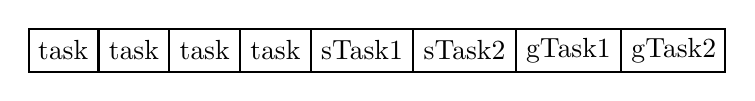
\begin{tikzpicture}[
  thick,
  myrect/.style={
    draw,
    rectangle split,
    rectangle split horizontal,
    rectangle split parts=#1,
    rectangle split part align=center
    } 
]

\node[myrect=8]
  {
  \nodepart{one}task
  \nodepart{two}task
  \nodepart{three}task
  \nodepart{four}task
  \nodepart{five}sTask1
  \nodepart{six}sTask2
  \nodepart{seven}gTask1
  \nodepart{eight}gTask2
  };

\end{tikzpicture}
\end{document}
	\caption{An example of the tasks and start and goal tasks seen as an array for an assembly with $4$ tasks and $2$ machines}
	\label{fig:tasks_array}
\end{figure}

\noindent We group together all tasks in one set in order for a more readable notation further down.
 \begin{equation}\label{eq:21}
 allTasks = tasks \cup startTasks \cup goalTasks
 \end{equation}

  \noindent Here we define the machines available for the assembly. A machine in this model is an arm.
 \begin{equation}\label{eq:2}
 nbrMachines \in \{1 , \ldots , 2^{32}-1\}
 \end{equation}
 \begin{equation}\label{eq:11}
 machines = \{1 , \ldots , nbrMachines\}
 \end{equation}

  \noindent These are the tools that can be fitted on an arm. The model assumes that there is a set of $nbrTools$ for each machine. I.e. if $nbrTools = 2$ and $nbrMachines = 2$, there is a set of tool $1$ and tool $2$ for machine $1$, and another set of tools $1$ and $2$ for machine $2$. There cannot be a combination of tools such as, for example, only tool $1$ for machine $1$ and a set of tools $1$ and $2$ for machine $2$.
 
 $toolNeeded(t)$ defines the tool that task $t$ needs.
 \begin{equation}\label{eq:3}
 nbrTools \in \{1 , \ldots , 2^{32}-1\}
 \end{equation}
 \begin{equation}\label{eq:12}
 tools = \{1 , \ldots , nbrTools\}
 \end{equation}
 \begin{equation}\label{eq:33}
 toolNeeded(t) \in tools, \; t \in tasks
 \end{equation} 

  \noindent $nbrComponents$ defines the number of components used. All components need to be uniquely identified in the assembly, so even if we use 4 screws in an assembly, we need to define all 4 screws. As mentioned before, we distinguish between components and \emph{primitve} components. The reason for this is that in the model we do not distinguish between a \emph{primitve} component and a sub-assembly, they are the same. And in the model we call them components. The reason for this is because we found it easier to only have one sort of object to deal with when it comes to what will be assembled, instead of two. This means that the final assembly is also a component, i.e. the product produced by the assembly is a component. In other words, in this thesis \emph{primitve} components and sub-assemblies are sub sets of components.
  
  $componentsUsed(t)$ defines the set of components task $t$ uses. A task usually only uses one component at a time, but uses two in the case of mounting tasks, the mounted component and the component mounted on.
  
  To know when a sub-assembly is created we set it as $compoentCreated$ for the task where it is created. This cannot happen anywhere else than in a mount task, although there is no check in the model for it. If no component is created in a task, $componentCreated=0$.
 \begin{equation}\label{eq:6}
 nbrComponents \in \{1 , \ldots , 2^{32}-1\}
 \end{equation}
 \begin{equation}\label{eq:13}
 components = \{1 , \ldots , nbrComponents\}
 \end{equation}
 \begin{equation}\label{eq:25}
 componentsUsed(t) \subset components, \; t \in tasks
 \end{equation}
 \begin{equation}\label{eq:componentCreated}
 componentCreated(t) \in components \cup \{0\}, \; t \in tasks
 \end{equation}

  \noindent Since components also can be sub-assemblies, it means a component can have subcomponents. These have been grouped in different groups to assist the constraints.

  $taskSubComponents(t)$ is the set of components that make up the subcomponents for the components used in task $t$. One can think of the subcomponents as layers with the component on top, call it origin component, and the layer below are the components that make up that component, and so on. $taskSubComponents(t)$ contains the components one layer down, if the component itself is not a \emph{primitve} component. In that case, $taskSubComponents(t)$ contains that component instead. See Figure \ref{fig:taskSubComponents} for an example.
 \begin{equation}\label{eq:53}
 taskSubComponents(t) \subset components, \; t \in tasks
 \end{equation}

 \begin{figure}
 \documentclass{standalone}
\usepackage{tikz}
\usetikzlibrary{positioning, calc}
\usepackage{standalone}
\usepackage{amsmath, amssymb}


\begin{document}
\begin{tikzpicture}[node distance=2cm,remember picture,
outer/.style={draw=black,thick,inner sep=5pt}]

\node(ex1){
\begin{tikzpicture}
\node[outer] (A) {
	\begin{tikzpicture}
		\node(task1){Task t1};
		\node[shape = ellipse,draw, below of=task1, yshift=1cm](tbr){Top-Button-Ring};
	\end{tikzpicture}
};

\node[outer, dashed, below of=A] (B) {
	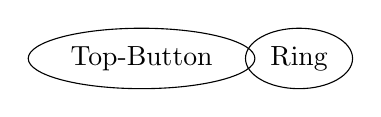
\begin{tikzpicture}
		\node[shape = ellipse,draw, solid](tb){Top-Button};
		\node[shape = ellipse,draw, right of=tb, xshift=1cm, solid](r){Ring};
	\end{tikzpicture}
};

\path[thick,->,>=stealth](tbr)edge(tb);
\path[thick,->,>=stealth](tbr)edge(r);
\end{tikzpicture}
};

\node[right of=ex1, xshift=5cm](ex2){
\begin{tikzpicture}
\node[outer] (A) {
	\begin{tikzpicture}
		\node(task1){Task t2};
		\node[shape = ellipse,draw, below of=task1, yshift=1cm](s1){Switch};
	\end{tikzpicture}
};

\node[outer, dashed, below of=A] (B) {
	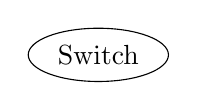
\begin{tikzpicture}
		\node[shape = ellipse,draw, solid](s2){Switch};
	\end{tikzpicture}
};

\path[thick,->,>=stealth](s1)edge(s2);
\end{tikzpicture}
};

\end{tikzpicture}
\end{document} 

 \caption{$taskSubComponents$ for two tasks, $t1$ and $t2$. $t1$ contains a sub-assembly, Top-Button-Nut, and $t2$ contains a primitive component, Switch. The $taskSubComponents$ for each task is shown in the dashed box beneath them.}
 \label{fig:taskSubComponents}
 \end{figure}
 
 \noindent To use the layer metaphor again, $taskCompleteSubComponents(t)$ contains all the layers below the origin component, for all the components in task $t$, not including the origin component itself. If the origin component is a \emph{primitve} component, the set is empty. See Figure \ref{fig:taskCompleteSubComponents} for an example.
 \begin{equation}\label{eq:54}
 taskCompleteSubComponents(t) \subset components, \; t \in tasks
 \end{equation}
 
  \begin{figure}
  \documentclass{standalone}
\usepackage{tikz}
\usetikzlibrary{positioning, calc}
\usepackage{standalone}
\usepackage{amsmath, amssymb}


\begin{document}
\begin{tikzpicture}[node distance=2cm,remember picture,
outer/.style={draw=black,thick,inner sep=5pt}]

\node(ex1){
\begin{tikzpicture}
\node[outer] (A) {
	\begin{tikzpicture}
		\node(task1){Task t1};
		\node[shape = ellipse,draw, below of=task1, yshift=1cm](tbr){Top-Button-Ring};
	\end{tikzpicture}
};

\node[outer, dashed, below of=A, yshift=-1cm] (B) {
	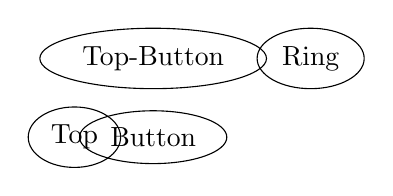
\begin{tikzpicture}
		\node[shape = ellipse,draw, solid](tb){Top-Button};
		\node[shape = ellipse,draw, solid, below of=tb, xshift=-1cm](t){Top};
		\node[shape = ellipse,draw, solid, right of=t](b){Button};
		\node[shape = ellipse,draw, right of=tb, xshift=1cm, solid](r){Ring};
	\end{tikzpicture}
};

\path[thick,->,>=stealth](tbr)edge(tb);
\path[thick,->,>=stealth](tb)edge(t);
\path[thick,->,>=stealth](tb)edge(b);
\path[thick,->,>=stealth](tbr)edge(r);
\end{tikzpicture}
};

\node[right of=ex1, xshift=5cm](ex2){
\begin{tikzpicture}
\node[outer] (A) {
	\begin{tikzpicture}
		\node(task1){Task t2};
		\node[shape = ellipse,draw, below of=task1, yshift=1cm](s1){Switch};
	\end{tikzpicture}
};

\node[outer, dashed, below of=A] (B) {
	\begin{tikzpicture}
		\node[shape = ellipse](s2){};
	\end{tikzpicture}
};

\path[thick,->,>=stealth](s1)edge(s2);
\end{tikzpicture}
};

\end{tikzpicture}
\end{document} 

  \caption{$taskCompleteSubComponents$ for two tasks, $t1$ and $t2$. One contains a sub-assembly, Top-Button-Nut, and the other contains a primitive component, Switch. The $taskCompleteSubComponents$ for each task is shown in the dashed box beneath them.}
  \label{fig:taskCompleteSubComponents}
  \end{figure}
 
  \noindent $subComponents(c)$ contains only the the \emph{primitve} subcomponents for component $c$, one layer down. If $c$ is a \emph{primitve} component or is only made of sub-assemblies, the set is empty.
 \begin{equation}\label{eq:55}
 subComponents(c) \subset components, \; c \in components
 \end{equation}

  \noindent Trays are used to hold components until we need them in the assembly. It can be that the tray holds the components from the beginning, as with \emph{primitve} components fed to the assembly, or it can be a sub-assembly put there during the assembly to be picked up again later. Each \emph{primitve} component has its own tray, so we can have a button tray, a cover tray, etc.
  
  $tray(t)$ is the tray task $t$ uses. If no tray is used by the task, $tray(t) = 0$.
 \begin{equation}\label{eq:4}
 nbrTrays \in \{1 , \ldots , 2^{32}-1\}
 \end{equation}
 \begin{equation}\label{eq:14}
 trays = \{1 , \ldots , nbrTrays\}
 \end{equation}
 \begin{equation}\label{eq:22}
 tray(t) \in trays \cup \{0\}, \; t \in tasks
 \end{equation}

  \noindent $fixtures$ defines the fixtures available in the assembly. A fixture is primarily used to hold a component in order for another component to be mounted on that component. Although, as was shown in the case study in chapter \ref{cha:assembly}, the fixture can be used for purposes other than just holding components.
  
  $fixture(t)$ is the fixture task $t$ uses. If no fixture is used by the task, $fixture(t) = 0$
 \begin{equation}\label{eq:5}
 nbrFixtures \in \{1 , \ldots , 2^{32}-1\}
 \end{equation}
 \begin{equation}\label{eq:15}
 fixtures = \{1 , \ldots , nbrFixtures\}
 \end{equation}
 \begin{equation}\label{eq:24}
 fixture(t) \in fixtures \cup \{0\}, \; t \in tasks
 \end{equation}

  \noindent $outputs$ defines the outputs available. An output is the final stage for a component in an assembly. After it is put here, it will not be removed. Although, there can still be other components mounted on the component put on the output. In that respect an output can be viewed as a fixture, only that the components put there can not be removed.
 
 $output(t)$ is the output used by task $t$. If no output is used by the task, $output(t) = 0$.
 \begin{equation}\label{eq:7}
 nbrOutputs \in \{1 , \ldots , 2^{32}-1\}
 \end{equation}
 \begin{equation}\label{eq:16}
 outputs = \{1 , \ldots , nbrOutputs\}
 \end{equation}
 \begin{equation}\label{eq:23}
 output(t) \in outputs \cup \{0\}, \; t \in tasks
 \end{equation}

  \noindent $concurrentTasks(k)$ is the $k$:th concurrent group among the concurrent groups defined. A concurrent group is a group of tasks that has to be performed at the same time. Hence, a concurrent group can not be larger than the amount of machines available, although, there is no check for it in the model. 
    
 \begin{equation}\label{eq:8}
 nbrConcurrentGroups \in \{1 , \ldots , 2^{32}-1\}
 \end{equation}
 \begin{equation}\label{eq:17}
 concurrentGroups = \{1 , \ldots , nbrConcurrentGroups\}
 \end{equation}
 \begin{equation}\label{eq:30}
 concurrentTasks(k) \subset tasks, \; k \in concurrentGroups
 \end{equation}

  \noindent $orderedGroup(k)$ is the $k$:th ordered group specified, there are $nbrOrderedGroups$ ordered groups. An ordered group is an array of tasks that have to come in a very specific order. An example of this could be if an assembly has many move tasks that need to be performed one after another in order to make some intricate movement. As seen in section \ref{seq:constraints}, we can reason about the relation between tasks if they use a certain component and are a certain kind of action. But we cannot reason about two move tasks, there is no way to tell which should come before the other based on the component they use. 
  
  $orderedGroup(k)$ is an array and the tasks in it will be scheduled in the order they come in the array. All the tasks in the group will be performed on the same machine.
  
  If one wants to access a certain task in a group, one can use $ordered(k,i)$ to access the $i$:th element of the $k$:th group.
  
  $orderedSet$ is the set of all tasks included in some ordered group.
 \begin{equation}\label{eq:900}
 nbrOrderedGroups \in \{1 , \ldots , 2^{32}-1\}
 \end{equation}
 \begin{equation}\label{eq:9}
 orderedGroups = \{1 , \ldots , nbrOrderedGroups\}
 \end{equation}
 \begin{equation}\label{eq:18}
 orderedGroup(k) \subset tasks, \; k \in orderedGroups
 \end{equation}
 \begin{equation}\label{eq:32}
 ordered(k,i) \in tasks, \; i \in \{1 , \ldots , |orderedGroup(k)|\}, \; k \in orderedGroups
 \end{equation}
 \begin{equation}\label{eq:39}
 orderedSet = \bigcup_{\forall k \in orderedGroups}orderedGroup(k), \; orderedSet \subset tasks
 \end{equation}

  \noindent $tray(t)$, $output(t)$ and $fixture(t)$ cannot be set at the same time for a task, since that would mean that the task is performed at two locations at the same time, although this is not checked by the model. The only restriction for what kind of tasks can be performed using these containers is that outputs cannot be used by take tasks and trays cannot be used by a mount tasks. If an assembly contains these combinations, the output or tray should be changed to a fixture.
 
  Each task performed can be classified as either a mount task, a take task, a move task or a put task, but only as one of them.
  \begin{description}
  \item[Taking] A task that picks up a component is a taking task. The location of the component is specified by either a tray or a fixture, but not an output since there is no reason to pick up something that has been placed on an output.
  
  \item[Mounting] A task that mounts a component on another component is a mounting task. This assumes that the component to mount is picked up and in the hand. The location of the component to mount on is defined by either a fixture or an output.
  
  \item[Putting] A task that puts a component somewhere is a putting task. Where a component is put is defined by either a fixture, a tray or an output.
  
  \item[Moving] A task that moves a component from one place to another is a moving task. The model already puts in moves between tasks and if, for example, the first task is a take task and the second task is a put task, the move in between them is essentially a move that moves a component from one place to the another. Although, sometimes it can be handy to define a task that explicitly moves a component. An example of that can be if one wants to spin a component around. Then one can specify a take task in order to pick up the component, a move task to turn it, and a put task to put the component back. In this case there will be three moves of the component; one to move from the take task to the move task, the move task itself, and a move from the move task to the put task.
   \end{description}
 \begin{equation}\label{eq:26}
 mounting \subset tasks
 \end{equation}
 \begin{equation}\label{eq:27}
 taking \subset tasks
 \end{equation}
 \begin{equation}\label{eq:28}
 moving \subset tasks
 \end{equation}
 \begin{equation}\label{eq:29}
 putting \subset tasks
 \end{equation}

  \noindent $putting(c)$, $mounting(c)$, $taking(c)$ and $moving(c)$ are subsets of respective set above based on the component involved.
 \begin{equation}\label{eq:35}
 putting(c) \subset putting, \; c \in components
 \end{equation}
 \begin{equation}\label{eq:36}
 mounting(c) \subset mounting, \; c \in components
 \end{equation}
 \begin{equation}\label{eq:37}
 taking(c) \subset taking, \; c \in components
 \end{equation}
 \begin{equation}\label{eq:38}
 moving(c) \subset moving, \; c \in components
 \end{equation}

  \noindent $duration(t)$ is simply the duration of task $t$.
 \begin{equation}\label{eq:42}
 duration(t) \in \{0 , \ldots , 2^{32}-1\}, \; t \in tasks
 \end{equation}
 
   \begin{figure}
   	\centering
    	\documentclass{standalone}
\usepackage{tikz}
\usetikzlibrary{calc, shapes, backgrounds}
\usepackage{standalone}
\usepackage{amsmath, amssymb}
\pagecolor{olive!50!yellow!50!white}
\begin{document}

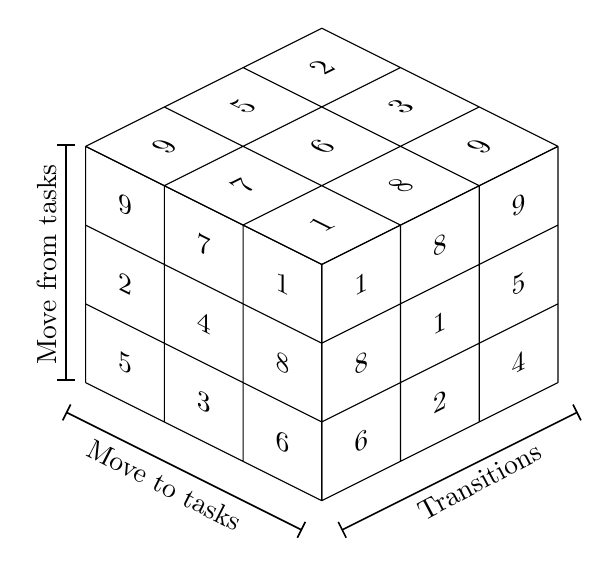
\begin{tikzpicture}
\begin{scope}[every node/.append style={yslant=-0.5},yslant=-0.5]
  \node at (0.5,2.5) {9};
  \node at (1.5,2.5) {7};
  \node at (2.5,2.5) {1};
  \node at (0.5,1.5) {2};
  \node at (1.5,1.5) {4};
  \node at (2.5,1.5) {8};
  \node at (0.5,0.5) {5};
  \node at (1.5,0.5) {3};
  \node at (2.5,0.5) {6};
  \draw (0,0) grid (3,3);
\end{scope}
\begin{scope}[every node/.append style={yslant=0.5},yslant=0.5]
  \node at (3.5,-0.5) {1};
  \node at (4.5,-0.5) {8};
  \node at (5.5,-0.5) {9};
  \node at (3.5,-1.5) {8};
  \node at (4.5,-1.5) {1};
  \node at (5.5,-1.5) {5};
  \node at (3.5,-2.5) {6};
  \node at (4.5,-2.5) {2};
  \node at (5.5,-2.5) {4};
  \draw (3,-3) grid (6,0);
\end{scope}
\begin{scope}[every node/.append style={
    yslant=0.5,xslant=-1},yslant=0.5,xslant=-1
  ]
  \node at (3.5,2.5) {9};
  \node at (3.5,1.5) {7};
  \node at (3.5,0.5) {1};
  \node at (4.5,2.5) {5};
  \node at (4.5,1.5) {6};
  \node at (4.5,0.5) {8};
  \node at (5.5,2.5) {2};
  \node at (5.5,1.5) {3};
  \node at (5.5,0.5) {9};
  \draw (3,0) grid (6,3);
\end{scope}

%x-axis
\draw[|-|,semithick,yslant=-0.5] (-0.25,-0.5) -- (2.75,-0.5);
\draw (1,-1.3) node[rotate= -27] {Move to tasks};

%y-axis
\draw[|-|,semithick,yslant=-0.5] (-0.25,-0.1) -- (-0.25,2.9);
\draw (-0.25,1.5) node[rotate=90, anchor= south] {Move from tasks};

%z-axis
\draw[|-|,semithick,yslant=-0.5] (3.25,-0.25) -- (6.25,2.75);
\draw (5,-1.25) node[rotate=28] {Transitions};
\end{tikzpicture}
\end{document} 

    	% or use \input{mytikz}
    	\caption{The timeMatrix3D}
    	\label{fig:3d_matrix}
   \end{figure}

\noindent For the model to decide how long a move between two tasks should take and whether there should be a change of tool in between, a matrix is used, $timeMatrix3D$, see Figure \ref{fig:3d_matrix}. This is a 3-dimensional matrix and contains the times for moving between all the tasks depending on what tool change occurs. On its y-axis it has the tasks to move from, on the x-axis the tasks to move to, and on the z-axis the different transitions between tools that can occur. There are $nbrMachines$ more rows on the y-axis than there are columns on the x-axis. This is because we also account for the starting position of the machines, so each start task has move times associated with them for moving to the other tasks. As the matrix is constructed the way it is, there is no move times between start tasks. 

 $timeMatrixDepth$ is the length of the z-axis, i.e. the depth of the matrix. It should be said that the reason for using the method described below is to reduce the size of the matrix and avoid redundancy.
 
 What we mean with ''different transitions'' is easiest shown through an example. Let us say we have $3$ tools available for each machine. We consider each tool state as a node in a graph, see Figure \ref{fig:tools_trans}, with the old tool state to the left and the new tool state to the right. Between them we can draw the different ways we can change state. The we start to consider which ones we actually need. We can change from tool $1$ to tool $1$, which is not changing tool at all. The same can be done for tool $2$, but not changing tool here costs just as much time as with tool $1$. So the change from tool $1$ to itself covers not changing tool for this tool, as well as for all the other tools, thereby we only need to keep track of one of these changes. We can also change from tool $1$ to tool $2$. And we can change back from $2$ to $1$, although here in the model we assume the change from one tool to another takes the same time the other way around as well. Therefore, we consider the change from tool $1$ to tool $2$ the same as from tool $2$ to tool $1$, and only keep track of one of them. If we keep considering the rest of the transitions this way, we will end up with a reduced number of transitions, in our case $4$, see Figure \ref{fig:tools_trans}
 
 It is clear that, $timeMatrixDepth$ obeys the equation (\ref{eq:timeMatrixDepth}). 
 \begin{equation}\label{eq:timeMatrixDepth}
 timeMatrixDepth = \frac{n^2 - n + 2}{2}, \; n = nbrTools
 \end{equation}
  \begin{equation}
  \begin{aligned}\label{eq:44}
  timeMatrix3D(t(from),t(to),k) &\in \{0 , \ldots , 2^{32}-1\},\\
  t(from) &\in tasks \cup startTasks,  \\ 
  t(to) &\in tasks, \; k \in \{0 , \ldots , timeMatrixDepth\}
  \end{aligned}
  \end{equation}

 
 \begin{figure}
 	\centering
 	\documentclass{standalone}
\usepackage{tikz}
\usetikzlibrary{calc, shapes, backgrounds}
\usepackage{standalone}
\usepackage{amsmath, amssymb}
\pagecolor{olive!50!yellow!50!white}
\begin{document}
\tikzset{
  leaf/.style = {draw=none,label = center:\textsf{$\vdots$}},
  labels/.style={midway, sloped, above, yshift=-10pt}
}
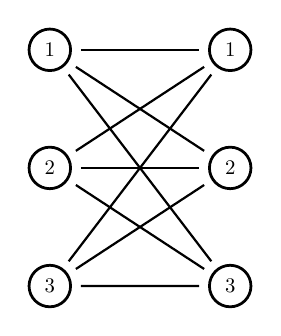
\begin{tikzpicture}
[
    scale = 0.75, transform shape, thick,
    every node/.style = {draw, circle, minimum size = 5mm, line width = 1pt, align=center},
    grow = down,  % alignment of characters
    level 1/.style = {sibling distance=6cm},
    level 2/.style = {sibling distance=2cm}, 
    level 3/.style = {sibling distance=1cm}, 
    level distance = 3 cm
  ]
  
  \tikzset{VertexStyle/.style = {shape          = circle,
                                   text           = black,
                                   inner sep      = 2pt,
                                   outer sep      = 5pt,
                                   minimum size   = 20pt}}
  \begin{scope}[node distance=20mm and 10mm]
  \node[VertexStyle](11){1};
  \node[VertexStyle, below of= 11](12){2};
  \node[VertexStyle, below of= 12](13){3};

  \node[VertexStyle, right= 2cm of 11](21){1};
  \node[VertexStyle, below of= 21](22){2};
  \node[VertexStyle, below of= 22](23){3};
  \end{scope}
  
  \draw(11) to (21);
  \draw(11) to (22);
  \draw(11) to (23);
  \draw(12) to (21);
  \draw(12) to (22);
  \draw(12) to (23);
  \draw(13) to (21);
  \draw(13) to (22);
  \draw(13) to (23);

\end{tikzpicture}
\end{document} 

  	\documentclass{standalone}
\usepackage{tikz}
\usetikzlibrary{calc, shapes, backgrounds}
\usepackage{standalone}
\usepackage{amsmath, amssymb}
\pagecolor{olive!50!yellow!50!white}
\begin{document}
\tikzset{
  leaf/.style = {draw=none,label = center:\textsf{$\vdots$}},
  labels/.style={midway, sloped, above, yshift=-10pt}
}
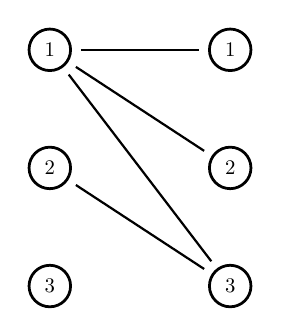
\begin{tikzpicture}
[
    scale = 0.75, transform shape, thick,
    every node/.style = {draw, circle, minimum size = 5mm, line width = 1pt, align=center},
    grow = down,  % alignment of characters
    level 1/.style = {sibling distance=6cm},
    level 2/.style = {sibling distance=2cm}, 
    level 3/.style = {sibling distance=1cm}, 
    level distance = 3 cm
  ]
  
  \tikzset{VertexStyle/.style = {shape          = circle,
                                   text           = black,
                                   inner sep      = 2pt,
                                   outer sep      = 5pt,
                                   minimum size   = 20pt}}
  \begin{scope}[node distance=20mm and 10mm]
  \node[VertexStyle](11){1};
  \node[VertexStyle, below of= 11](12){2};
  \node[VertexStyle, below of= 12](13){3};

  \node[VertexStyle, right= 2cm of 11](21){1};
  \node[VertexStyle, below of= 21](22){2};
  \node[VertexStyle, below of= 22](23){3};
  \end{scope}
  
  \draw(11) to (21);
  \draw(11) to (22);
  \draw(11) to (23);
  \draw(12) to (23);

% \node (Start){}
%   child {   node [] (A) {}
%     child { node [] (D) {}
%       child { node [leaf] (M) {}}
%       child { node [leaf] (N) {}}
%     }
%     child { node [] (E) {}
%       child { node [leaf] (O) {}}
%       child { node [leaf] (P) {}}
%     }
%     child { node [] (F) {}
%       child { node [leaf] (Q) {}}
%       child { node [leaf] (R) {}}
%     }
%   }
%   child {   node [] (B) {}
%     child { node [] (G) {}
%       child { node [leaf] (S) {}}
%       child { node [leaf] (T) {}}
%     }
%     child { node [] (H) {}
%       child { node [leaf] (U) {}}
%       child { node [leaf] (V) {}}
%     }
%     child { node [] (I) {}
%       child { node [leaf] (X) {}}
%       child { node [leaf] (Y) {}}
%     }
%   }
%   child{ node(C){}
%     child { node [] (J) {}
%       child { node [leaf] (Z) {}}
%       child { node [leaf] (A1) {}}
%     }
%     child { node [] (K) {}
%       child { node [leaf] (B1) {}}
%       child { node [leaf] (C1) {}}
%     }
%     child { node [] (L) {}
%       child { node [leaf] (D1) {}}
%       child { node [leaf] (E1) {}}
%     }
%   };
\end{tikzpicture}
\end{document} 

  	\caption{All the transitions between the tool states to the left. The reduced number of transitions between the tool states to the right}
  	\label{fig:tools_trans}
 \end{figure}

\noindent Depending on the physical layout of the assembly, sometimes not all the tasks can be done by all machines. It could be that the machines would collide or simply that the spatial location is out of reach for the machine. In those cases we can specify that tasks are out of hand for a specific machine. This is the only time when we distinguish between the two machines and connect the machine in the model model with the machine in the real world. In all other aspects the machines in the model are identical and have the potential to perform the same work.
 \begin{equation}\label{eq:56}
 taskOutOfRange(m) \subset tasks, \; m \in machines
 \end{equation}
 
 
 \subsection{Decision variables}
 Decision variables are variables that can take many values. It is these values that the solver sets out to determine in order to solve the problem.

  \noindent The model has to decide which task uses which machine.
 \begin{equation}\label{eq:40}
 usingMachine(t) \in machines, \; t \in tasks
 \end{equation}

  \noindent Each task has a predecessor that tells the model what other task comes right before the task in question on the same machine.
 \begin{equation}\label{eq:41}
 pred(t) \in allTasks, \; t \in allTasks
 \end{equation}

  \noindent In order to create an upper limit for variables dealing with time, we create a rough upper limit of the complete assembly. It simply takes the longest duration for a task and the longest duration for a move between tasks and assert it for all the tasks.
 \begin{equation}
 \begin{aligned}\label{eq:maxE}
 maxE = &(max(\{duration(t) : t \in tasks\}) \; +  \\ 
 &\begin{aligned}
 max(\{&timeMatrix3D(t_1,t_2,k) : \\
 &\forall t_1 \in tasks \cup startTasks,  \\ 
 &\forall t_2 \in tasks,\\
 &\forall k \in \{0 , \ldots , timeMatrixDepth\}\}) \times nbrTasks
  \end{aligned}
 \end{aligned}
 \end{equation}

  \noindent Each task has to have a start time. We set it to be anywhere between time $0$ and the maximum possible end calculated before.
 
 To simplify notation we also introduce one more variable called $end(t)$. It is the time when task $t$ ends and is simply the sum of the start and the duration of the task.
 \begin{equation}\label{eq:46}
 start(t) \in \{0 , \ldots , maxE\}, \; t \in allTasks
 \end{equation} 
 \begin{equation}\label{eq:47}
 end(t) = start(t) + duration(t), \; t \in allTasks
 \end{equation}

  \noindent As mentioned before, each task has a move time connected to it since it takes a certain amount of time to move from one task to another. Since this time depends on both what task comes before it and what tools are needed for both of the tasks, the duration for the move is a decision variable as opposed to the duration for the task itself.
 \begin{equation}\label{eq:49}
 moveDuration(t) \in \{0 , \ldots , maxE\}, \; t \in allTasks
 \end{equation}
 \begin{equation}\label{eq:50}
 moveStart(t) \in \{0 , \ldots , maxE\}, \; t \in allTasks
 \end{equation}
 \begin{equation}\label{eq:51}
 moveEnd(t) = moveStart(t) + moveDuration(t), \; t \in allTasks
 \end{equation}

  \noindent Since the goal of the assembly is to complete the assembly in as little time as possible, we set up a variable for it, $makespan$. It is this variable the solver will try to minimize.
 \begin{equation}\label{eq:48}
 makespan \in \{0 , \ldots , maxE\}
 \end{equation}

  \noindent The last variable is for determine what tool should be used for a task. With $toolNeeded$ we specify what tool is needed for the specific task. But we do not need to specify a tool if the task does not need any specific tool. That is why we need to determine what tool should be used for those tasks. Leaving the option open by not specifying any particular tool opens up for optimisations since it could mean we can avoid costly tool changes.
 \begin{equation}\label{eq:52}
 toolUsed(t) \in tools, \; t \in allTasks
 \end{equation}
  
 
 \section{Constraints}\label{seq:constraints}
 In this section some of the most important constraints for the model will be described. For a full list of used constraints see \emph{Appendix A}, while for the MiniZinc code see \emph{Appendix B}.
 \\\\
 $makespan$ should represent the total time of the whole assembly. That means it should be equal to the largest end time among all the tasks. We can enforce that by limiting the end time for each task to be less or equal to the $makespan$.
 \begin{equation}\label{eq:92}
 (\forall t \in tasks) \; end(t) \le makespan
 \end{equation}

  \noindent Start and goal tasks are special tasks since they act as source and sink nodes. This means they never get scheduled in time as ordinary tasks, we set them to all start at time $0$ and they do not have a duration variable, since the do not take up any time. We also assign them to machines so each start and goal task pair have their own machine from the start.
 \begin{equation}\label{eq:93}
 (\forall t \in startTasks \cup goalTasks) \; start(t) = 0
 \end{equation}
 \begin{equation}
 \begin{aligned}\label{eq:94}
 (\forall m \in machines) \; usingMachine(nbrTasks + m) &= m\\
 \land \; usingMachine(nbrTasks + nbrMachines + m) &= m
 \end{aligned}
 \end{equation}

  \noindent We enforce the $tasksOutOfRange(m)$ variables by simply saying that the tasks in the variable can not be assigned the machine $m$.
 \begin{equation}\label{eq:95}
 (\forall m \in machines) \; (\forall t \in tasksOutOfRange(m)) \; usingMachine(t) \neq m
 \end{equation}

  \noindent As said before, the $toolNeeded$ contains what tool is needed for a task. We need to translate it into what tool is used. It is done by simply taking the value from $toolNeeded$ and assigning it to $toolUsed$ for the tasks where a tool is specified, i.e. $toolNeeded$ is not $0$.
 \begin{equation}\label{eq:117}
 (\forall t \in tasks, \; toolNeeded(t) \neq 0) \; toolUsed(t) = toolNeeded(t)
 \end{equation}

 
 \subsection{Precedences}
 These constraints deals with the order in time in which the tasks have to come.

  \noindent A very fundamental part of the relation between a task and the move to it is that we cannot start a task before we have moved to it.
  \begin{equation}\label{eq:107}
  (\forall t \in tasks) \; Start(t) \geq moveEnd(t)
  \end{equation}

  \noindent If we want to mount two components together, we first have to put the first component in a fixture before we can mount the other component on it. Hence, the put task has to end before we can start with the mount task. 
 \begin{equation}
 \begin{aligned}\label{eq:96}
 (\forall comp &\in components) \\
 (\forall mountTask &\in mounting(comp)) \\
 (\forall putTask &\in putting(comp)) \\
 end(putTask) &\le moveStart(mountTask)
 \end{aligned}
 \end{equation}

  \noindent In the case mentioned above we also have take tasks for both components and they must both be performed before we can start mounting anything.
 \begin{equation}
 \begin{aligned}\label{eq:97}
 (\forall comp &\in components) \\
 (\forall mountTask &\in mounting(comp)), \\
 (\forall takeTask &\in taking(comp)), \\
 end(takeTask) &\le moveStart(mountTask)
 \end{aligned}
 \end{equation}

  \noindent Say we want to put a component away for a while and pick it up again later. Then we need to do that in a tray. This is the only time we put anything in a tray, usually we just take components from them. So we can apply the (\ref{eq:98}) constraint which says that if there is a take and a put on the same tray, then the take has to happen after the put. 
 \begin{equation}
 \begin{aligned}\label{eq:98}
 (\forall comp &\in components) \\
 (\forall putTask &\in putting(comp), \; tray(putTask) > 0)\\
 (\forall takeTask &\in taking(comp), \; tray(putTask) = tray(takeTask))\\
 end(putTask) &\le moveStart(takeTask)
 \end{aligned}
 \end{equation}

  \noindent When there is a put task and a take task on a fixture where a sub-component of the component being taken is the component being put, the put task has to happen before the take task.
 \begin{equation}
 \begin{aligned}\label{eq:99}
 (\forall f &\in fixtures) \\
 (\forall putTask &\in putting, \; fixture(putTask) = f)\\
 (\forall takeTask &\in taking, \; fixture(takeTask) = f \; \land \\
 &componentsUsed(putTask) \subset taskSubComponents(takeTask)) \\
 end(putTask) &\le moveStart(takeTask), \\
 \end{aligned}
 \end{equation}

  \noindent Since we can do many sub-assemblies on the same fixture, we need to ensure that if a component is put in the fixture, there cannot be a component from another sub-assembly put or mounted there before the sub-assembly is done.
  
  We can observe that the task of doing a sub-assembly begins with a put of a component in a fixture and a take of a component from the same fixture. The taken component will have the put component as a sub-component. With this knowledge we start by extracting all put tasks for a fixture. Then we extract all the corresponding take tasks, i.e. the take tasks for that fixture where the component used in the put task is among the sub-components for the component in the take task. Although, there is the case where we construct a component by first doing some mounting, then we take it up to maybe turn it or fixate it, and then put it back in the fixture for further mounting. In this case we will get two takes matching with the first put. So we need to identify which take task is the first one. We do this by choosing the take task with the least amount of subcomponents.
  
  Now we have a 1:1 matching of take tasks and put tasks. To ensure the time between when a put task occurs and when the take task occurs, we apply a \emph{cumulative} constraint over that time and the limit of the fixture is always $1$.
  
  When $[$ and $]$ are used together with $:$ as below, it means they are array generators. What is left of the $:$ is what is put in the array and what is right of it is the condition. A case here which might be confusing is the last argument to the cumulative constraint. It simply states that it is an array of ones with the same length as $puts$.
 \begin{equation}
 \begin{aligned}\label{eq:100}
 &(\forall f \in fixtures) \\
 &puts = [put : put \in putting, \; fixture(put) = f], \\
 &\begin{aligned}
 takes = [min(\{&take : take \in taking, \; fixture(take) = f,\\ &componentsUsed(put) \subset taskCompleteSubComponent(take)\}) : \\
 &put \in puts], 
 \end{aligned}\\
 &\begin{aligned}
 cumulative(&[moveStart(task) : task \in puts], \\ &[abs(end(takes(i))-moveStart(puts(i))) : i \in \{1 , \ldots , |puts|\}], \\
 &[1 : i \in \{1 , \ldots , |puts|\}],\\
 &1)
 \end{aligned}\\
 \end{aligned}
 \end{equation}

  \noindent The fundamental property of the tasks in a concurrent group is that they need to execute at the same time on different machines. We ensure this with (\ref{eq:101}).
 \begin{equation}
 \begin{aligned}\label{eq:101}
 (\forall group &\in \{1 , \ldots , nbrConcurrentGroups\}) \\
 (\forall t_1 &\in concurrentTasks(group)) \\
 (\forall t_2 &\in concurrentTasks(group) \setminus \{t_1\}) \\
 start(t_1) &= start(t_2) \; \land \\
 usingMachine(t_1) &\neq usingMachine(t_2), \\
 \end{aligned}
 \end{equation}

  \noindent A very logical observation we can do is that components cannot be used before they are created. This is enforced in (\ref{eq:102}).
 \begin{equation}
 \begin{aligned}\label{eq:102}
 (\forall t_1 &\in tasks, \; componentCreated(t_1) > 0) \\
 (\forall t_2 &\in tasks, \; componentCreated(t_1) \in componentUsed(t_2)) \\
 moveStart(t_2) &\geq end(t_1) \\
 \end{aligned}
 \end{equation}

  \noindent A similar observation as for (\ref{eq:102}) is that we have to perform all tasks with a component before it is part of a sub-assembly. Therefore we can say that all tasks need to have an end time smaller than the start time of the tasks having the tasks component as sub-component.
 \begin{equation}
 \begin{aligned}\label{eq:103}
 (\forall precTask &\in tasks) \\
 (\forall t &\in tasks, \; precTask \neq t,\\
 &componentUsed(precTask) \cup taskCompleteSubComponents(t) \\
 &\subset taskCompleteSubComponents(t),\\
 &componentsUsed(precTask) \cup taskCompleteSubComponents(t) \neq \emptyset)\\
 end(precTask) &\leq moveStart(t), \\
 \end{aligned}
 \end{equation}

  \noindent Trays, fixtures and outputs can only be used one at a time. We can rephrase this into saying that tasks using trays cannot overlap, tasks using fixtures cannot overlap, etc. We ensure this by applying the \emph{cumulative} constraint through (\ref{eq:104}), (\ref{eq:105}) and (\ref{eq:106}).
 \begin{equation}
 \begin{aligned}\label{eq:104}
 &\begin{aligned}
 (\forall f &\in fixtures) \\
 fixtureTasks &= [t : t \in tasks, \; fixture(t) = f], 
 \end{aligned}\\
 &\begin{aligned}
 cumulative(&[start(t) : t \in fixtureTasks],\\
 &[duration(t) : t \in fixtureTasks],\\
 &[1 : t \in fixtureTasks],\\
 &1)
 \end{aligned}\\
 \end{aligned}
 \end{equation}
 \begin{equation}
 \begin{aligned}\label{eq:105}
 &\begin{aligned}
 (\forall tr &\in trays) \\
 trayTasks &= [t : t \in tasks, \; tray(t) = tr], 
 \end{aligned}\\
 &\begin{aligned}
 cumulative(&[start(t) : t \in trayTasks],\\
 &[duration(t) : t \in trayTasks],\\
 &[1 : t \in trayTasks],\\
 &1)
 \end{aligned}\\
 \end{aligned}
 \end{equation}
 \begin{equation}
 \begin{aligned}\label{eq:106}
 &\begin{aligned}
 (\forall o &\in outputs) \\
 outputTasks &= [t : t \in tasks, \; output(t) = o], \\
 \end{aligned}\\
 &\begin{aligned}
 cumulative(&[start(t) : t \in outputTasks], \\
 &[duration(t) : t \in outputTasks], \\
 &[1 : t \in outputTasks], \\
 &1)
 \end{aligned}\\
 \end{aligned}
 \end{equation}

 
 \subsection{Predecessors}
 All tasks need to have a predecessor that tells the model what task comes directly before it on the same machine. This means that a task can only have one predecessor. It can be seen as the way a machine needs to travel through its tasks in order to complete the assembly, where we have a start task at the start and a goal task at the end. If we were to connect the start and the goal task we wold have a circuit, hence we could view each machine as a circuit. And we could model each machine as a circuit, but then we would need to synchronise all the sub-circuits and ensure that tasks only appeared in one sub-circuit. This would make for quite a few constraints and would make the model more complex. Instead we model all the machines as one circuit and we tie together the goal task of one sub-circuit with the start task of the next for each sub-circuit, to form a large circuit. Then we tie together the goal task of the last sub-circuit with the start task of the first, see (\ref{eq:110}). Lastly we can apply the \texttt{circuit} constraint over all $pred$ variables.
  
 The attentive reader might have observed that the nodes in the \texttt{circuit} constraint have successors and not predecessors. Even if it is the wrong way around, it does not matter if the constraint sees the predecessor variable as a successor or a predecessor, it will form a circuit anyway.
 
 \begin{equation}\label{eq:109}
 \begin{aligned}
 (\forall startTask &\in startTasks \setminus \{nbrTasks + 1\}) \\
 pred(startTask) &= startTask + nbrMachines - 1
 \end{aligned}
 \end{equation}
 \begin{equation}\label{eq:110}
 pred(nbrTasks + 1) = nbrTasks + nbrMachines \times 2
 \end{equation}
 \begin{equation}\label{eq:111}
 circuit(\{pred(t) : \forall t \in tasks\})
 \end{equation}

  \noindent A fundamental part of a predecessor is that it is the task directly before the task in question, therefore the predecessor has to end before the task starts, or more specific, even before the move to the task.
 \begin{equation}\label{eq:108}
 (\forall t \in tasks) \; moveStart(t) \geq end(pred(t))
 \end{equation}

  \noindent  Another fundamental part is that a predecessor is a task performed on the same machine as the task in question. This is enforced by (\ref{eq:115}).
 \begin{equation}\label{eq:115}
 \begin{aligned}
 (\forall t &\in tasks \cup goalTasks) \\
 usingMachine(t) &= usingMachine(pred(t)) 
 \end{aligned}
 \end{equation}

  \noindent In a sense, the ordered groups are forced predecessors and hence we enforce that by simply by making a task predecessor to the next task in the array.
 \begin{equation}
 \begin{aligned}\label{eq:114}
 &\begin{aligned}
 (\forall k &\in orderedGroups) \\
 (\forall i &\in \{1 , \ldots , |orderedGroup(k)|-1\}) 
 \end{aligned}\\
 &pred(ordered(k, i + 1)) = ordered(k, i) \\
 \end{aligned}
 \end{equation}

  \noindent The following two constraints can seem very specific, but are essential to the scheduling in our model.
\\\\
 In order to properly connect the taking of a component and the mounting of one, we need to ensure that if there is no put task, the take task has to be the predecessor of the mount task. 
 
 But we must also ensure the following: The put cannot be on the same fixture or output as the mount. This is because a component that will be mounted in a fixture or output will always first be picked up, then put in either a fixture or output, then mounted with with another component. The component mounted on will also be part of the mounting task. Therefore, if the component is the one being mounted, there will be two tasks; one where the component is taken, and one where the component is mounted. And that is no problem, the constraint applies. But if the component is the one being mounted on, there will be three tasks; one where the component is taken, one where the component is put in a fixture or output, and one where it is mounted on. In this case the take task cannot be the predecessor of the mount task, since the component first must be put in the fixture or output, and then the other take task,  where the component being mounted on this component is taken, should be the predecessor of the mount task. Hence we ensure there are no put tasks working on the same fixture or output as the mount task.
 
 The final case we must consider is when there are move tasks involved. There can be a case of a take task of a component, then a couple of move tasks, and lastly a mount task. In this case, the take task cannot be the predecessor of the mount task, and this constraint does not apply. If we applied it, it would contradict the (\ref{eq:114}) constraint. So we need to ensure that the take task is not in an ordered group either.
 \begin{equation}
 \begin{aligned}\label{eq:112}
 (\forall c &\in components) \\
 (\forall mountTask &\in mounting(c)) \\
 puts &= \{p : p \in putting(c),\\
 &(fixture(p) > 0 \land fixture(p) = fixture(mountTask)) \\
 &\lor \; (output(p) > 0 \land output(p) = output(mountTask))\}, \\
 (\forall takeTask &\in taking(c), \; takeTask \notin orderedSet, \; puts = \emptyset) \\
 pred(mountTask) &= takeTask \\
 \end{aligned}
 \end{equation}

  \noindent As with (\ref{eq:112}), in order to ensure the relation between when a component is picked up and when it is put that the take task is the predecessor of the put task, i.e. we must first pick up the components before we put it down, and there cannot be anyu other task in between.
  
  Also as with (\ref{eq:112}), there are a few cases to consider. If we want to put a component away for a while in order to pick it up later, there will be a put task and a take task on that component. But in this case the take task cannot come before the put task, since we need to put it down before we can pick it up. So we put in the clause that this constraint does not apply if the put task is on a tray.
  
  We also need to consider the occurrence of move tasks. If there is a move task involved between the take and put, the take task cannot be the predecessor of the put task.
 \begin{equation}
 \begin{aligned}\label{eq:113}
 (\forall c &\in components, \; moving(c) = \emptyset)\\
 (\forall putTask &\in putting(c), \; tray(putTask) = 0)\\
 (\forall takeTask &\in taking(c))\\
 pred(putTask) &= takeTask
 \end{aligned}
 \end{equation}

  \noindent (\ref{eq:116}) is the constraint that decides if there should be a tool change or not between two tasks. It first calculates what tool state transition will occur between the two tasks, $k$, by taking the difference between what tool is used in the task and its predecessor. If they use the same tool, no transition needs to occur, i.e. no tool change needed and the difference would be $0$. We add $1$ to $k$ since the indexes start at $1$ in \emph{MiniZinc} and a result of $0$ should take constraint to the first index dept-wise in the $timeMatrix3D$.
 \begin{equation}\label{eq:116}
 \begin{aligned}
 (\forall t &\in tasks) \\
 k &= abs(toolUsed(t) - toolUsed(pred(t))) + 1, \\
 moveDuration(t) &= timeMatrix3D(pred(t), \; t, \; k)
 \end{aligned}
 \end{equation}
 
 \newpage
 
 \section{Filter}
  In \cite{VilimBartak2002Batch} \cite{Vilim2002Precedence} \cite{VilimBartak2002Sequence} Vilím shows that filtering the domains of variables when, as in our case, using sequence dependent setup times can have a great effect on the runtime. Here we present a set of filters in order to minimize the domains of the variables.
  
\subsection{Temporal filter}
  The largest domains in the model are the domains for the variables dealing with time, i.e. the temporal variables. Reducing those has the potential to cut much of the processing time.
  \\\\
   We start with defining two variables, $maxMoveDurs(t)$ and $minMoveDurs(t)$. These contain the maximum duration and the minimum duration, respectively, for each task taken from the time matrix.
  \begin{equation}
  \begin{aligned}\label{eq:57}
  &( \forall t \in tasks)\\
  &\begin{aligned}
  maxMoveDurs(t) = max(\{&timeMatrix3D(t,j,k) :\\
  &\forall j \in tasks, \\
  &\forall k \in \{1 , \ldots , timeMatrixDepth\},\\
  &j \neq t\})
  \end{aligned}
  \end{aligned}
  \end{equation}
   \begin{equation}
   \begin{aligned}\label{eq:58}
   &(\forall t \in tasks)\\
   &\begin{aligned}
   minMoveDurs(t) = min(\{&timeMatrix3D(t,j,k) :\\
   &\forall j \in tasks, \\
   &\forall k \in \{1 , \ldots , timeMatrixDepth\},\\
   &j \neq t\})
   \end{aligned}
   \end{aligned}
   \end{equation}

  \noindent By using the newly created variables we can -*define yet another two. These define a new maximum for the total time of the assembly, $maxEnd$. It is similar to $maxE$ in equation (\ref{eq:maxE}), although much more thorough in the filtering. These variables also define a new minimum for the total time of the assembly, it was earlier ju set to 0.
   
   To calculate the maximum end we look at the worst case scenario for the assembly. The worst case would be if all the tasks had to be done one after the other, one at a time, on the same machine and they would take the longest time, according to the time matrix, to move between them. See Figure \ref{fig:worst_case}. This can simply be defined by summing the durations and maximum move durations for all the tasks.
   
   To calculate the minimum end we look at the best case scenario. The best case scenario is if all the tasks can be evenly scheduled over all machines, taking the shortest, according to the time matrix, time to move between them. See Figure \ref{fig:best_case}. We can define this by summing up the durations and minimum move durations for all the task end divide the sum with the number of machines available. If the tasks can be perfectly evenly scheduled across all the machines, the total assembly time will be equal to $minEnd$, if they cannot $minEnd$ will always be smaller than the total assembly time.
  \begin{equation}\label{eq:59}
 	maxEnd = \sum_{\forall t \in tasks} duration(t) + maxMoveDurs(t)
  \end{equation}
  \begin{equation}\label{eq:minEnd}
  	minEnd = \frac{\sum_{\forall t \in tasks} duration(t) + minMoveDurs(t)}{nbrMachines}
  \end{equation}

 
  \begin{figure}
  	\centering
  	\documentclass{standalone}
\begin{document}

\sffamily
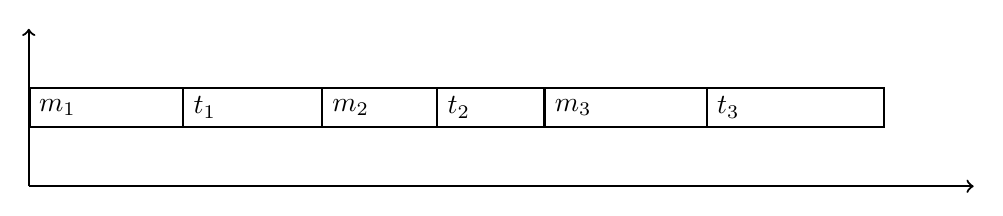
\begin{tikzpicture}[
  thick,
  myrect/.style={
    draw,
    rectangle split,
    rectangle split horizontal,
    rectangle split parts=#1,
    rectangle split part align=center
    } 
]

\node[myrect=6, anchor=west](assembly)
  {
  \nodepart[text width= 17mm]{one}$m_1$
  \nodepart[text width= 15mm]{two}$t_1$
  \nodepart[text width= 12mm]{three}$m_2$
  \nodepart[text width= 11mm]{four}$t_2$
  \nodepart[text width= 18mm]{five}$m_3$
  \nodepart[text width= 20mm]{six}$t_3$
  };
  
      % Draw axes
      \draw[thick,->] (0,-1) -- (0,1);
      \draw[thick,->] (0,-1) -- (12,-1);

\end{tikzpicture}

\end{document} 

  	% or use \input{mytikz}
  	\caption{The worst case assembly}
  	\label{fig:worst_case}
  \end{figure}
   \begin{figure}
   	\centering
   	\documentclass{standalone}
\begin{document}

\sffamily
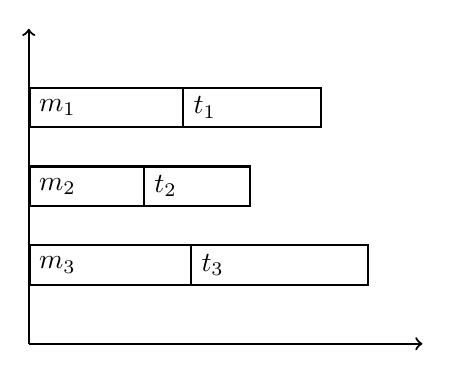
\begin{tikzpicture}[
  thick,
  myrect/.style={
    draw,
    rectangle split,
    rectangle split horizontal,
    rectangle split parts=#1,
    rectangle split part align=left
    } 
]

\node[myrect=2,anchor=west](assembly)
  {
  \nodepart[text width= 17mm]{one}$m_1$
  \nodepart[text width= 15mm]{two}$t_1$
  };
  
\node[myrect=2, below =of assembly.west,anchor=west](assembly2)
  {
  \nodepart[text width= 12mm]{one}$m_2$
  \nodepart[text width= 11mm]{two}$t_2$
  };
  
\node[myrect=2, below=of assembly2.west,anchor=west](assembly3)
  {
  \nodepart[text width= 18mm]{one}$m_3$
  \nodepart[text width= 20mm]{two}$t_3$
  };
  
      % Draw axes
      \draw[thick,->] (0,-3) -- (0,1);
      \draw[thick,->] (0,-3) -- (5,-3);

\end{tikzpicture}

%\begin{tikzpicture}
%\tikzset{VertexStyle/.style = {anchor= west, draw, align= center, text height= 2.5mm}
%}
%
%    % Draw axes
%    \draw [<->,thick] (0,4) node (yaxis) [above] {}
%        |- (45mm,0) node (xaxis) [right] {};
%
%   \node[VertexStyle, text width= 15mm] (rect1) at (0mm,3)  {$m_1$};
%   \node[VertexStyle, text width= 15mm] (rect2) at (18mm,3) {$t_1$};
%   
%   \node[VertexStyle, text width= 10mm] (rect1) at (0mm,2)  {$m_2$};
%   \node[VertexStyle, text width= 11mm] (rect2) at (13mm,2) {$t_2$};
%      
%   \node[VertexStyle, text width= 11mm] (rect1) at (0mm,1)  {$m_3$};
%   \node[VertexStyle, text width= 20mm] (rect2) at (14mm,1) {$t_3$};
%\end{tikzpicture}
\end{document} 

   	% or use \input{mytikz}
   	\caption{The best case assembly}
   	\label{fig:best_case}
   \end{figure}
 
 \noindent We can now start using $maxEnd$ and $minEnd$ to filter variables
 \\\\
  We set and upper bound for the start of a task by setting it to happen at latest the duration of the task time units before the $maxEnd$, since the task has to have time to execute before the end.
  
  To set a lower bound for the start of a task, we simply reason that the move to the task can start at its earliest at time 0. Therefore, we limit the task to start earliest direct after the minimum move duration to it.
  
  The difference between (\ref{eq:lim_start_over}) and (\ref{eq:lim_start_under}) is that the upper limit can be set for all sorts of tasks, even the start and goal tasks, but the lower limit cannot be set for start and goal tasks. This is simply because the start and goal tasks do not have any move times to them since they are source and sink nodes.
  \begin{equation}\label{eq:lim_start_over}
  \begin{aligned}
 &(\forall t \in allTasks)\\
 &start(t) \le maxEnd-duration(t)
  \end{aligned}
  \end{equation}
   \begin{equation}\label{eq:lim_start_under}
  \begin{aligned}
 &(\forall t \in Tasks)\\
 &start(t) \ge minMoveDurs(t)
  \end{aligned}
  \end{equation}

\newpage

  \noindent In order to limit the move start to a task we use the same reasoning as with start. But now we have to account for that there comes a task after the move and a duration of the move itself. So we have to subtract the duration of the task and the duration of the move. Since we do not know the exact length of the move, we have to use the value we know the duration can not be lower than, which is $minMoveDuration$.
  \begin{equation}\label{eq:63}
  (\forall t \in tasks) \; moveStart(t) \le maxEnd-(duration(t)+minMoveDurs(t))
  \end{equation}

  \noindent  We have already calculated the limits for the whole assembly, $maxEnd$ and $minEnd$. Now we just enforce them on the makespan.
  \begin{equation}\label{eq:66}
  \begin{aligned}
  makeSpan &\le maxEnd \land\\
  makespan &\ge minEnd
  \end{aligned}
  \end{equation}

   \noindent The first thing that has to happen to a component in the assembly is that is has to be picked up. So since the assembly starts out with empty machines the first thing that has to happen, with the exception of a tool change, is a take task. Therefore, we can limit that start of the tasks not being take tasks to happen at earliest after the task with the smallest sum of duration and minimum move duration.
  \begin{equation}
  \begin{aligned}\label{eq:69}
  &(\forall t \in tasks \setminus taking) \\
  &moveStart(t) \ge min(\{duration(tt) + minMoveDurs(tt) : \forall tt \in taking\})
  \end{aligned}
  \end{equation}

  \noindent  The start of a task can be even further limited by analysing the components used by the task and how that relates to what components are created by other tasks.
    
    Lets take task $t$ as an example. We start by getting all tasks that create the components that are used in task $t$, $prevTasks$. These tasks have to come before task $t$ since the component that they create cannot be used before they are created. If the number of machines is greater than or equal to the number of task preceding task t, then the best scheduling that can be done is to do all tasks in parallel. That means that task $t$ can start at earliest after the one of the preceding tasks taking the longest to complete.
  \begin{equation}
  \begin{aligned}\label{eq:70}
  &(\forall t \in tasks)\\
  &\begin{aligned}
  prevTasks = \{task : \; &task \in tasks,\\
  &componentCreated(task) \in componentsUsed(t)\},
  \end{aligned}\\
  &\begin{aligned}
  nbrMachines &\ge |prevTasks|,\\
  0 &< |prevTasks|,
  \end{aligned}\\
  &start(t) \ge max(\{duration(pt) + minMoveDurs(pt) : \forall pt \in prevTasks\}) \\
  \end{aligned}
  \end{equation}

   \noindent But if the number of machines is fewer than the number of preceding tasks, the best we can do is divide them as equally as possible over the machines. This is the same reasoning as when we calculated $minEnd$ in equation (\ref{eq:minEnd}).
  \begin{equation}
  \begin{aligned}\label{eq:71}
  &(\forall t \in tasks) \\
  &\begin{aligned}
  prevTasks(t) = \{task : \; & task \in tasks,\\
  &componentCreated(task) \in componentsUsed(t)\},
  \end{aligned} \\
  &nbrMachines < |prevTasks(t)|,  \\
  &start(t) \ge \frac{\left(\sum_{\forall pt \in prevTasks(t)}duration(pt) + minMoveDurs(pt)\right)}{nbrMachines}
  \end{aligned}
  \end{equation}

   \noindent To set the upper limit for the start of tasks we use a little bit different strategy.
    
    We know that if a component $c$ has been mounted on another component, $c$ cannot be used again on its own. Therefore, a task that uses component $c$ has to come before the tasks that uses a component in which $c$ is a part of.
    
    We use the same strategy as in (\ref{eq:70}) and look at the best case scenario where the tasks are performed concurrently on all machines. The difference here from (\ref{eq:70}) is that here we have to look at the maximum end of the assembly and subtract the successor task which takes the longest to perform and the duration of the task in question.
  \begin{equation}\label{eq:72}
  \begin{aligned}
  &(\forall t \in tasks) \\
  &succTasks(t) = \{task : \; task \in tasks,\\
  &componentsUsed(t) \subset taskCompleteSubComponent(task)\}, \\
  &\begin{aligned}
  nbrMachines &\ge |succTasks(t)|,\\
  0 &< |succTasks(t)|,
  \end{aligned}\\
  &\begin{aligned}
  start(t) \le maxEnd - max(\{&duration(st) + minMoveDurs(st) :\\
  &\forall st \in succTasks(t)\}) - duration(t)
  \end{aligned}\\
  \end{aligned}
  \end{equation}

  \noindent  As with (\ref{eq:71}) we look at the worst case scenario.
  \begin{equation}\label{eq:73}
  \begin{aligned}
  &(\forall t \in tasks)\\
  &succTasks = \{task : \; task \in tasks, \\
  &componentsUsed(t) \subset taskCompleteSubComponent(task)\}, \\
  &nbrMachines \le |succTasks|, \\
  &\begin{aligned}
  start(t) \; \le \; &maxEnd - \frac{\left(\sum_{\forall st \in succTasks}duration(st) + minMoveDurs(st)\right)}{nbrMachines}\\
  &- duration(t)
  \end{aligned}
  \end{aligned}
  \end{equation}

  
  
  \subsection{Predecessor filter}
  Since the predecessors are searched by the solver before searching the start variables, reducing their domains has the potential to help reduce the total runtime considerably.
 \\\\
  In our model the tools can only pick up one component at a time. This also means that if a task puts down a component or mounts one, there cannot be a mount or put task directly afterwards.
  \begin{equation}\label{eq:75}
  (\forall t1, \forall t2 \in taking) \; pred(t1) \neq t2
  \end{equation}
  \begin{equation}\label{eq:76}
  (\forall t1, \forall t2 \in putting \cup mounting) \; pred(t1) \neq t2
  \end{equation}
\newpage
   \noindent Using a similar reasoning as in (\ref{eq:72}) and (\ref{eq:73}), we can find the tasks that cannot be the predecessor of task $t$. We look at what tasks uses the components that has the components used in $t$ as sub-components. This means that those components cannot come before task $t$, and therefore cannot be predecessors of $t$.
  \begin{equation}
  \begin{aligned}\label{eq:78}
  &(\forall t \in tasks)\\
  &nonPredecessors(t) = \{t_2 : \; t_2 \in tasks, \\
  &componentsUsed(t) \subset taskCompleteSubComponents(t_2) \; \lor \\
  &componentsUsed(t) \subset subComponents(componentCreated(t_2))\} \\
  &(\forall nonPred \in nonPredecessors(t)) \\
  &pred(t) \neq nonPred, \\
  \end{aligned}
  \end{equation}

   \noindent As mentioned before, a component has to be picked up first before it can be manipulate in any way and the assembly has to start with a take task. Therefore, we can say that an assembly cannot start with neither a put task nor a mount task.
    
    The same could be said for move tasks, but since they need to be in an ordered group, a constraint like these would make no difference.
  \begin{equation}\label{eq:79}
  \begin{aligned}
  &(\forall startTask \in startTasks)\\
  &(\forall putTask \in putting)\\
  &pred(putTask) \neq startTask
  \end{aligned}
  \end{equation}
  \begin{equation}\label{eq:80}
   \begin{aligned}
   &(\forall startTask \in startTasks)\\
   &(\forall mountTask \in mounting)\\
   &pred(mountTask) \neq startTask 
   \end{aligned}
  \end{equation}

   \noindent The same way we can observe that an assemble needs to start with a take task, we can observe that an assembly cannot end with a take task. There is no component in the assembly that does not end up in the finished assembly, therefore the assembly cannot end with a machine holding a component, since it needs to be on the output in some way.
  \begin{equation}\label{eq:81}
  \begin{aligned}
  &(\forall goalTask \in goalTasks) \\
  &(\forall takeTask \in taking) \\
  &pred(goalTask) \neq takeTask
  \end{aligned}
  \end{equation}
 
  \noindent Continuing the reasoning around what tasks can come first and not we can expand with which tasks have to come last. We cannot limit the last task on each arm to be on an output, because it does not necessarily need to be that. Although, among the last tasks in the assembly there needs to be a task on an output. We can easily check that by placing a constraint over the $pred$ variables for the goal tasks. This is what (\ref{eq:82}) says.
   
   We can do the same reasoning with what needs to come first in the assembly. As we stated before, a take task has to be the first task in the assembly. And as with the last tasks in the assembly, the first task of a machine does not have to be a take task, but there needs to be at least one take task among the first tasks. We ensure this in (\ref{eq:83}) by placing a constraint over the $pred$ variables for the take tasks.
  \begin{equation}
  \begin{aligned}\label{eq:82}
  &\begin{aligned}
  counts &= [i : \; task \in outputTasks, \; i \in \{0 , \ldots , 1\}], \\
  outputTasks &= [task : \; task \in tasks, \; output(task) > 0], \\
  goalPreds &= [pred(task) : \; task \in goalTasks],
  \end{aligned} \\
  &global\_cardinality(goalPreds, \; outputTasks, \; counts)\\
  &\land \; \sum counts > 0
  \end{aligned}
  \end{equation}
   \begin{equation}
   \begin{aligned}\label{eq:83}
   &\begin{aligned}
   counts &= [i : \forall task \in startTasks, \; i \in \{0 , \ldots , 1\}], \\
   takePreds &= [pred(task) : \forall task \in taking], \\
   startTasksArray &= [task : \; task \in startTasks], 
   \end{aligned}\\
   &global\_cardinality(takePreds, \; startTasks, \; counts) \\
   &\land \; \sum counts > 0
   \end{aligned}
   \end{equation}
   
   \section{Heuristics}
   The search was declared to go over the variables through a sequential search\\\cite{mz_tute} in the following order:
   
   \begin{enumerate}
   \item The $usingMachine$ variables
   \item The predecessor variables for take tasks that are not on an output
   \item The predecessor variables for put tasks that are not on an output
   \item The predecessor variables for mount tasks that are not on an output
   \item The predecessor variables for tasks that are on an output
   \item The predecessor variables in general
   \item The start times of the tasks
   \end{enumerate}
   
   The branching heuristics chosen in the searches 1-6 above was \texttt{indomain\_median}. This means the median value of the domain will be chosen to branch on. This is because there is no numerical relationship between the value the variables can take and the order in which they should come. If constructing the MiniZinc data file using \texttt{AssemblyConv}, see appendix \ref{app:tool_manuals}, the values of the variables depends on the order in which entities are declared. For search 7 above, the heuristic is \texttt{indomain\_min}, which means the smallest value of the domain will be chosen to branch on. This heuristic is chosen since the values of the start variables are the ones we want to minimize, so we search from the bottom up.

\chapter{Case Study}\label{cha:assembly}
In order to develop and test the model, we have chosen to focus on one representative case study. In this case study the robot is assembling an enclosed emergency stop button used in industrial environments, see Figure \ref{fig:button}. The assembly is presented in \cite{assembly} and has an associated video of the assembly\footnote{\url{http://www.youtube.com/watch?v=7JgdbFW5mEg}}. Please note that this is not the video used to extract the times for the tasks, so the times may differ from the ones used. Also, only the assembly of one stop button is performed in this thesis, not several as in this video.

This assembly is composed of 5 components; a top, a button, a nut, a switch and a bottom. A combination of components that is not the complete assembly we will call a sub-assembly. The button needs to be inserted in the top and then the nut needs to be screwed onto the underside of the button in order to secure it to the top. The switch needs to be mounted in the bottom and, lastly, the top part, with button and nut, needs to be mounted on the bottom with the switch. In Figure \ref{fig:assembly} we see the top-button-nut assembly to the right and the bottom-switch assembly to the left. Note that the screws in the figure are not part of the case study assembly.

\begin{figure}
\centering
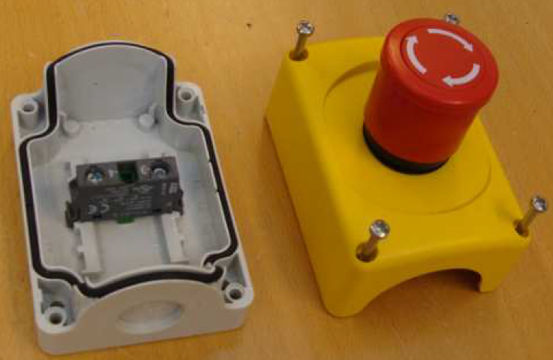
\includegraphics[width=\textwidth/3*2]{Figures/buttonbox.png}
\caption{Picture of the button used in the case study. The screws are not part of the case study assembly}
\label{fig:button}
\end{figure}

The assembly includes objects such as trays and fixtures. A tray is a holder where components reside until they are needed in the assembly. A fixture is a holder in which components can be put so that another components can be mounted on it.

21 steps have been identified as needed for the assembly and they are taken from a video of an existing assembly created by hand. For an illustration of the order of the assembly steps, see Figure \ref{fig:assembly} The steps are as follows:

\begin{description}
\item[Take top] Takes the top component from its tray

\item[Put top in fixture] Puts the taken top component in a fixture

\item[Take button] Takes the button component from its tray

\item[Mount button on top] Mounts the taken button component onto the top component in a fixture

\item[Angle top-button] Angles the sub-assembly that is the top and button component, from here on called top-button, so it can be supported by the other machine.

\item[Lift top-button, hold top button] Lifts the top-button by holding the button

\item[Lift top-button, support] Lifts the top-button by supporting the top from underneath

\item[Turn top-button] Turns the top-button by holding the button

\item[Take nut] Takes the nut from its tray

\item[Mount nut on top-button, hold] Mounts the nut on top-button while holding the button

\item[Mount nut on top-button, mount] Mounts the nut on the top-button holding and screwing the nut. The sub-assembly created by the top-button and the nut is here on after called top-button-nut

\item[Fixate top-button-nut] Fixates the top-button-nut using the side of a fixture in order to get it straight.

\item[Put top-button-nut in top tray] The top-button-nut is put in the top tray in order to put it away for a while to be picked up later.

\item[Take top-button-nut from top tray] Takes the top-button-nut from the top tray where it was previously put.

\item[Take bottom] Takes the bottom component from its tray.

\item[Put bottom in fixture] Puts the bottom component in a fixture.

\item[Take switch] Takes the switch component from its tray.

\item[Mount switch in bottom] Mounts the switch on the bottom in the fixture the bottom was put in. The sub-assembly created here will be called bottom-switch.

\item[Take bottom-switch] Takes the created bottom-switch from the fixture.

\item[Put bottom-switch on table] Puts the bottom-switch on the table.

\item[Mount top-button-nut on bottom-switch] Mounts the top-button-nut on the button-switch on the table.
\end{description}

\noindent Most of the steps are self explanatory, but there are a few steps which are quite special that might need some more explanation. In steps \textbf{Mount nut on top-button, hold} and \textbf{Mount nut on top-button, mount} the button component has been put in the hole of the top and needs to secured using the nut component. To do we utilize somthing that is special for YuMi\textsuperscript\textregistered, using both arms in order to mount the nut. This is done mid air with one arm holding the top-button by gripping the button part, having it upside-down compared to how it was in the fixture, and with the other arm screwing the nut in place. The preparation for this starts at the end of step \textbf{Mount button on top}, where the sub-assembly top-button was just created, but the button is only loosely sitting in the hole of the top. The sub-assembly is angled in task \textbf{Angle top-button} about 45$^\circ$ in order to create a gap under the sub-assembly so the other arm can reach under the sub-assembly and help lift it from the fixture in tasks \textbf{Lift top-button, support} and \textbf{Lift top-button, hold top button}. Finally the top-button is rotated by only holding it with one arm in the button part of the sub-assembly and are now ready for the nut to be mounted.
It should be noted that since the operations of lifting the top-button and mounting the nut takes two arms and we have here split the operations into two tasks each, one for each arm, the tasks \textbf{Mount nut on top-button, hold} and \textbf{Mount nut on top-button, mount} needs to be performed at the same time. The same goes for  \textbf{Lift top-button, support} and \textbf{Lift top-button, hold top button}.

As mentioned before, the steps listed are taken from a video of an assembly. This makes the times used in the case study approximated. First the times where approximated using seconds as the unit of time. But it showed to be hard to approximate some of the tasks as they sometimes where under 1 second. Because of this and to get better print outs of the assembly using \texttt{SchedPrinter} (see appendix \ref{app:tool_manuals}) we multiplied the times we could estimate well from the video by 5 and approximated the other tasks as well as we could. This means that the real times for the tasks in the case study, and in the files mentioned in appendix \ref{app:tool_manuals}, are $1/5$ of the time presented. Because of this, comparing the time from the solvers with the time of the manual assembly is harder. We had to approximate the time of the manual assembly using the times we have approximated. By analysing the video and using the approximated times we got a time of 516 time units for the manual assembly.

\begin{landscape}
\begin{figure}
\documentclass{standalone}
\usepackage{standalone}
\begin{document}
\tikzstyle{task} = [rectangle, minimum width=3cm, minimum height=1cm, text centered, draw=black]
\tikzstyle{arrow} = [thick,->,>=stealth]
\begin{tikzpicture}[node distance=2cm]
\node (1) [task] {Take top};
\node (2) [task, right of=1, xshift=2.5cm] {Put top in fixture};

\node (3) [task, below of=1] {Take button};
\node (4) [task, below of=2] {Mount button on top};

\node (5) [task, xshift=2.5cm, right of=4] {Angle top-button};

\node (6) [task, right of=5, xshift=3cm, yshift=1cm] {Lift top-button, hold};
\node (7) [task, below of=6] {Lift top-button, support};

\node (8) [task, right of=7, xshift=3.5cm, yshift=1cm] {Turn top-button};

\node (10) [task, below of=8] {Mount ring, hold};
\node (11) [task, below of=10] {Mount ring, mount};

\node (9) [task, below of=11] {Take ring};

\node (12) [task, left of=11, xshift=-4cm, yshift=1cm] {Fixate top-button-ring};

\node (13) [task, left of=12, xshift=-9.5cm] {Put top-button-ring in top tray};
\node (14) [task, below of=13] {Take top-button-ring from top tray};

\node (15) [task, below of=9, yshift=-1.5cm] {Take switch};
\node (16) [task, left of=15, xshift=-3cm] {Mount switch};

\node (17) [task, below of=15] {Take bottom};
\node (18) [task, below of=16] {Put button in fixture};

\node (19) [task, left of=16, xshift=-3.5cm] {Take button-switch};

\node (20) [task, left of=19, xshift=-5cm] {Put bottom-switch on table};

\node (21) [task, above of=20] {Mount top-button-ring on bottom-switch};

\draw [arrow] (1) -- (2);
\draw [arrow] (3) -- (4);
\draw [arrow] (2) -- (4);
\draw [arrow] (4) -- (5);
\draw [arrow] (5) -- (6);
\draw [arrow] (5) -- (7);
\draw [arrow] (7) -- (8);
\draw [arrow] (6) -- (8);
\draw [arrow] (8) -- (10);
\draw [arrow] (10) -- (12);
\draw [arrow] (9) -- (11);
\draw [arrow] (11) -- (12);
\draw [arrow] (12) -- (13);
\draw [arrow] (13) -- (14);
\draw [arrow] (15) -- (16);
\draw [arrow] (17) -- (18);
\draw [arrow] (18) -- (16);
\draw [arrow] (16) -- (19);
\draw [arrow] (19) -- (20);
\draw [arrow] (20) -- (21);
\draw [arrow] (14) -- (21);

\end{tikzpicture}
\end{document}
\caption{The case study assembly}
\label{fig:assembly}
\end{figure}
\end{landscape}

%\documentclass{standalone}
\begin{document}
\begin{table}
\centering
\begin{tabular}{c|l|p{6cm}}
Step & Name                                  & Comment\\
\hline
1   & Take top                               & Takes the top component from its tray\\
2   & Put top in fixture                     & Puts the taken top component and puts it in a fixture\\
3   & Take button                            & Takes the button component from its tray\\
4   & Mount button on top                    & Mounts the taken button component onto the top component in a fixture\\
5   & Angle top-button                       & Angles the assembly that is the top and button component, from here on called top-button\\
6   & Lift top-button, hold top button       & Lifts the top-button by holding the button\\
7   & Lift top-button, support               & Lifts the top-button by supporting the top from underneath\\
8   & Turn top-button                        & Turns the top-button by holding the button\\
9   & Take ring                              & Takes the ring from its tray\\
10  & Mount ring on top-button, hold         & Mounts the ring on top-button by holding the button\\
11  & Mount ring on top-button, mount        & Mounts the ring on the top-button holding and screwing the ring. The assembly created by thetop-button and the ring is here on after called top-button-ring\\
12  & Fixate top-button-ring                 & Fixates the \\
13  & Put top-button-ring in top tray        &\\
14  & Take top-button-ring from top tray     &\\
15  & Take bottom                            &\\
16  & Put bottom in fixture                  &\\
17  & Take switch                            &\\
18  & Mount switch in bottom                 &\\
19  & Take bottom-switch                     &\\
20  & Put bottom-switch on table             &\\
21  & Mount top-button-ring on bottom-switch &\\
\end{tabular}
\caption{Steps in case study}\label{tab:assembly_steps}
\end{table}
\end{document}
\chapter{Evaluation}\label{cha:eval}
Here we will present the evaluation of the model. The focus of the test will be on retrieving the optimal solution from the solvers. This is when the solver has reached a solution and ended the search, thereby concluding that the last reached conclusion was the optimal. Each solver was given a time limit of 4 hours to complete the search as it seemed long enough to have a high probability of retrieving a result from all the solver, but short enough to be manageable to test. But as can be seen in section \ref{sec:res}, this was not always the case. In the case where the solvers could produce a result in the given time frame the solvers where run 10 times and the average time was used. But the optimal solution is maybe not always the goal of the assembly or not feasible in any reasonable time. The case could be such that one has a certain amount of time at hand and want to get a good assembly in that amount of time. Therefore we will also present information for the solvers that did not end the search within the given time but produced solutions, some even the optimal.

Originally, the 1.6 version of MiniZinc was used. But during the making of the model version 2.0 was released. According to NICTA, the 2.0 version is a complete rewrite of the MiniZinc-to-FlatZinc comipiler but that the resulting FlatZinc file is compatile with 1.6 solvers, and therefore no changes should be required for the solvers \cite{mz2}. We therefore thought it could be of interest to compare how the 2.0 version performed compare to the 1.6 version. During the test phase of the thesis version 2.0.1 was released that should fix some bugs in 2.0 \cite{mz2_changelog}. Therefore, version 2.0.1 is used.

Apart from measuring the time, we also analysed the resulting FlatZinc file to see if we could see any correlation between the running time and the data run. The data extracted was the number of integer and boolean variables, the number of arrays, the number of constraints and the percentage of constraints that were reified. We measure the reifieds since even if we try to avoid direct reifieds in the MiniZinc code, the FlatZinc could still contain reified constraints depending on how it translates the MiniZinc code.

In order to see if the filtering we introduced made any difference, we also measure the different combinations of the filters and the absence of filters. Because of all the combinations of parameters we want to test, there will be 8 test cases for each solver.

What we want to achieve is to get the solver to reach the optimal solution and conclude that it is the optimal solution, that is what we mean when we say \emph{result}. And it should be noted that the result is only analysed in comparison to the handmade assembly, so it will not be tested on an actual physical robot.

\section{The Setup}
The computer used to run the solvers was equipped with an Intel i7 2.8GHz quad core CPU, 8GB DDR3 1333MHz memory and running Mageia 4.
\\\\
The versions of each of the solvers are presented in the table below.
\begin{table}[h]
\centering
\begin{tabular}{l|l}
Solver                    & Version \\ \hline
G12/FD                    & 1.6.0\\
JaCoP                     & 4.2 \\
Gecode                    & 4.3.2 \\
or-tools                  & Rev. 3782 \\
Opturion CPX              & 1.0.2 \\
\multirow{2}{*}{Chcoco 3} & Solver: 3.2.2 \\
                          & Parser: 3.2.0
\end{tabular}
\end{table}\\\\
Note that for Choco3, the solver and parser has different version numbers. This is because they are not distributed together and therefore have slightly different version numbers. It is possible to specify the number of cores used by the solver for Gecode, or-tools and Choco3. Hence, these three were given access to all 4 cores when running.

The versions of the solvers used are the latest as of December 2014.

\section{The results}\label{sec:res}
The time for the assembly reached by the solvers as the optimal was 512 time units. This is the time we will use as the optimal when we henceforth talk about which solvers reached the optimal but did not finish the search.

The results presented in the tables \ref{tab:res_g12} to \ref{tab:res_choco} are the runtimes of the solvers and the analysis of the FlatZinc files. The tests are grouped into 4 categories of runs; with predecessor filter and temporal filter, with only predecessor filter, with only temporal filter and with no filter at all. In each of these groups there are two groups, one for each version we tests, i.e. MiniZinc 1.6 and 2.0.1.

For the solvers that did not end their search in the 4 hour time limit but still produced results we present the number of solutions reached in the 4 hours, \emph{\# solutions}. When a value is marked with a asterisk(*) it means the solver also reached the optimal solution in that time.

In the tables presented the filter names has been shortened to \emph{Pred} and \emph{Temp}. \emph{Pred} means the predecessor filter and \emph{Temp} means the temporal filter. We will also use two additional notations in the rime rows; "-" and "!". "-" means that the run did not complete within the given time frame. "!" means that the solver raised an error when reading the FlatZinc file.

The runtime will be presented in two formats, milliseconds and \emph{hours:minutes:seconds}, in the latter the remaining milliseconds are omitted.


\documentclass{standalone}
\begin{document}
\begin{table}[H]
\footnotesize
\centering
\begin{tabular}{lc|c|c|c|c|c|c|c}
\multicolumn{9}{c}{G12/FD} \\ 
\hline\hline Filter & \multicolumn{2}{c|}{Pred \& Temp} &\multicolumn{2}{c|}{Pred}  & \multicolumn{2}{c|}{Temp} & \multicolumn{2}{c}{None} \\ 
\hline Version & 1.6 & 2.0.1 & 1.6 & 2.0.1 & 1.6 & 2.0.1 & 1.6 & 2.0.1 \\ 
Time (ms)               & - & - & - & - & - & - & - & - \\
Time                    & - & - & - & - & - & - & - & - \\ 
\# of integer variables & 174 & 293 & 174 & 314 & 154 & 270 & 154 & 291 \\ 
\# of boolean variables & 162 & 97 & 162 & 97 & 142 & 106 & 142 & 106 \\ 
\# of arrays            & 31 & 53 & 31 & 53 & 29 & 51 & 29 & 51 \\ 
\# of constraints       & 2437 & 588 & 983 & 588 & 2153 & 562 & 699 & 562 \\ 
\% reified               & 7.50\% & 15.81\% & 18.61\% & 15.81\% & 7.57\% & 16.90\% &23.31\% & 16.90\% \\ 
\end{tabular}
\caption{Results for G12/FD}\label{tab:res_g12}
\end{table} 
\end{document}

\documentclass{standalone}
\begin{document}
\begin{table}[H]
\footnotesize
\begin{tabular}{lc|c|c|c|c|c|c|c}
\multicolumn{9}{c}{JaCoP} \\ 
\hline\hline Filter & \multicolumn{2}{c|}{Pred \& Dom} &\multicolumn{2}{c|}{Pred}  & \multicolumn{2}{c|}{Dom} & \multicolumn{2}{c}{None} \\ 
\hline Version & 1.6 & 2.0.1 & 1.6 & 2.0.1 & 1.6 & 2.0.1 & 1.6 & 2.0.1 \\ 
Time (ms)               & 635 & - & 1139619 & - & - & - & - & - \\ 
\# of integer variables & 129 & 223 & 129 & 244 & 129 & 229 & 129 & 250 \\ 
\# of boolean variables & 42 & 27 & 42 & 27 & 42 & 27 & 42 & 27 \\ 
\# of arrays            & 31 & 46 & 31 & 46 & 29 & 43 & 29 & 43 \\ 
\# of constraints       & 2318 & 425 & 781 & 425 & 2046 & 416 & 509 & 416 \\ 
\% refeid               & 2.71\% & 6.35\% & 8.06\% & 6.35\% & 3.07\% & 6.49\% & 12.37\% & 6.49\% \\ 
\end{tabular} 
\end{table}
\end{document}

\documentclass{standalone}
\begin{document}
\begin{table}[H]
\footnotesize
\centering
\begin{tabular}{lc|c|c|c|c|c|c|c}
\multicolumn{9}{c}{Opturion CPX - no warm start} \\ 
\hline\hline Filter & \multicolumn{2}{c|}{Pred \& Dom} &\multicolumn{2}{c|}{Pred}  & \multicolumn{2}{c|}{Dom} & \multicolumn{2}{c}{None} \\ 
\hline Version & 1.6 & 2.0.1 & 1.6 & 2.0.1 & 1.6 & 2.0.1 & 1.6 & 2.0.1 \\ 
Time (ms)               &    -     & !       & -       & !       & -       & !       & -       & !       \\ 
Time                    &    -     & !       & -       & !       & -       & !       & -       & !       \\ 
\# of integer variables & 28736    & 9531    & 28736   & 28876   & 28716   & 9508    & 28716   & 28853	  \\ 
\# of boolean variables & 57284    & 18654   & 57284   & 57322   & 57264   & 18702   & 57264   & 57370	  \\ 
\# of arrays            & 31       & 4698    & 31      & 14370   & 29      & 4714   & 29      & 14386	  \\ 
\# of constraints       & 102402   & 33025   & 100947  & 100679  & 102117  & 33028   & 100663  & 100682  \\ 
\% reified               & 55.98\%  & 56.25\% & 56.78\% & 56.85\% & 56.11\% & 56.24\% & 56.92\% & 56.85\% \\ 
\end{tabular}
\caption{Results for Opturion CPX}\label{tab:res_cpx}
\end{table}
\end{document}

\documentclass{standalone}
\begin{document}
\begin{table}[H]
\footnotesize
\centering
\begin{tabular}{lc|c|c|c|c|c|c|c}
\multicolumn{9}{c}{Gecode} \\ 
\hline\hline Filter & \multicolumn{2}{c|}{Pred \& Temp} &\multicolumn{2}{c|}{Pred}  & \multicolumn{2}{c|}{Temp} & \multicolumn{2}{c}{None} \\ 
\hline Version & 1.6 & 2.0.1 & 1.6 & 2.0.1 & 1.6 & 2.0.1 & 1.6 & 2.0.1 \\ 
Time (ms)               & - & 60 & - & 71761 & - & 99 & - & 71186 \\ 
Time                    & - & 0:00:00 & - & 0:01:11 & - & 0:00:00 & - & 0:01:11 \\ 
\# of integer variables & 129 & 225 & 129 & 246 & 129 & 230 & 129 & 251 \\ 
\# of boolean variables & 42 & 27 & 42 & 27 & 42 & 27 & 42 & 27 \\ 
Total \# of variables   & 171 & 252 & 171 & 273 & 171 & 257 & 171 & 278 \\ 
\# of arrays            & 30 & 57 & 30 & 57 & 28 & 50 & 28 & 50 \\ 
\# of constraints       & 2193 & 425 & 739 & 425 & 1951 & 420 & 497 & 420 \\ 
\% reified               & 2.87\% & 6.35\% & 8.52\% & 6.35\% & 3.22\% & 6.42\% & 12.67\% & 6.42\% \\ 
\end{tabular}
\caption{Results for Gecode}\label{tab:res_gecode}
\end{table}
\end{document}

\documentclass{standalone}
\begin{document}
\begin{tabular}{lc|c|c|c|c|c|c|c}
\multicolumn{9}{c}{or-tools} \\ 
\hline\hline Filter & \multicolumn{2}{c|}{Pred \& Dom} &\multicolumn{2}{c|}{Pred}  & \multicolumn{2}{c|}{Dom} & \multicolumn{2}{c}{None} \\ 
\hline Version & 1.6 & 2.0.1 & 1.6 & 2.0.1 & 1.6 & 2.0.1 & 1.6 & 2.0.1 \\ 
Time (ms)               & 257 & ! & 672 & ! & 564 & ! & 600 & ! \\ 
\# of integer variables & 129 & 223 & 129 & 244 & 129 & 229 & 129 & 250 \\ 
\# of boolean variables & 42 & 27 & 42 & 27 & 42 & 27 & 42 & 27 \\ 
\# of arrays            & 31 & 50 & 31 & 50 & 29 & 43 & 29 & 43 \\ 
\# of constraints       & 2316 & 421 & 779 & 421 & 2046 & 416 & 509 & 416 \\ 
\% refeid               & 2.72\% & 6.41\% & 8.08\% & 6.41\% & 3.07\% & 6.49\% & 12.37\% & 6.49\% \\ 
\end{tabular} 
\end{document}

\documentclass{standalone}
\begin{document}
\begin{tabular}{lc|c|c|c|c|c|c|c}
\multicolumn{9}{c}{Choco3} \\ 
\hline\hline Filter & \multicolumn{2}{c|}{Pred \& Dom} &\multicolumn{2}{c|}{Pred}  & \multicolumn{2}{c|}{Dom} & \multicolumn{2}{c}{None} \\ 
\hline Version & 1.6 & 2.0.1 & 1.6 & 2.0.1 & 1.6 & 2.0.1 & 1.6 & 2.0.1 \\ 
Time (ms)               & - & - & - & - & - & - & - & - \\ 
\# of integer variables & 129 & 223 & 129 & 244 & 129 & 229 & 129 & 250 \\ 
\# of boolean variables & 42 & 27 & 42 & 27 & 42 & 27 & 42 & 27 \\ 
\# of arrays            & 31 & 50 & 31 & 50 & 29 & 43 & 29 & 43 \\ 
\# of constraints       & 2316 & 421 & 779 & 421 & 2046 & 416 & 509 & 416 \\ 
\% refeid               & 2.47\% & 6.41\% & 8.08\% & 6.41\% & 3.07\% & 6.49\% & 12.37\% & 6.49\% \\ 
\end{tabular} 
\end{document}

If one just does a quick comparison of the numbers in the tables without doing any deeper analysis, one can see that the results from Gecode, or-tools and Choco3, shown in tables \ref{tab:res_gecode}, \ref{tab:res_or} and \ref{tab:res_choco}, respectively, are identical. This hints that the FlatZinc files for these solvers should be very similar. And indeed, if one compares the FlatZinc files for these three solvers for one of the cases, they are as good as identical. The difference between them is the naming of some constraints and sometimes the placement in the file.

As can be seen in the times or the runs, not many of the runs completed in time. Only 9 runs completed by 3 solvers. Interesting to note is the very varying runtimes. It ranges from 60 milliseconds to 16 minutes. Almost no solver could solve the problem using MiniZinc 2.0.1, two of them threw errors reading the FlatZinc file, despite its claimed backwards compatibility, and most others took too long time solving it. But, interestingly Gecode manages to solve the problem using 2.0.1, even faster than using 1.6, and even being the fastest to solve the problem of all the runs in just 60 milliseconds.
\\\\
By our definition of a result, these are the runs that found the optimal solution and ended the search by concluding that the optimal solution was found. This means that there are other runs that still produced results, sometimes even the optimal one, but did not end the search in time and therefore not qualify as a result.

The G12/FD runs using predecessor and temporal filter with version 2.0.1, using predecessor filter with version 1.6 and using predecessor filter with version 2.0.1 all find solutions, although none of them are the optimal.

The JaCoP runs using predecessor and temporal filter with version 2.0.1 and using predecessor filter with version 2.0.1 both finds all the solutions, including the optimal solution, immediately. This is also the case for JaCoP using predecessor filter with version 1.6.

The Gecode run using predecessor filter with version 2.0.1 finds three solution immediately of which one is the optimal. Interestingly, the run using no filter also with version 2.0.1 finds only one solution and that one is the optimal in roughly the same time.

The Choco3 runs using the predecessor and temporal filters and the ones using predecessor filter, independent of version, all finds two solutions immediately.

We should mention that some of the tests ran for much longer than the time limit set at 4 hours. And although not all produced results even when left for more than 4 hours, some managed to produce results. One that could be mentioned is Opturion CPX that in some cases took around 6 hours to complete.

We should also mention that Opturion CPX has the option to use the search strategy "warm start". This was tested but, as with regular complete search, did not produce a result within the time frame and thus we have not specifically included the results here.
\\\\
We will present some more tables that show the change in the values. The first 4 columns are grouped by the version of MiniZinc and in each of those groups we show the change in the values if each of the filters are added. The last column shows the change in values if going from using the 1.6 version to using the 2.0.1 version. The values presented are averages. For example, the change for when adding the temporal filter for version 1.6 is the average of the changes from not using any filters to using the temporal filter and from using the predecessor filter to using the temporal and predecessor filters. The average for the last column is just the average of the changes for all cases when switching from 1.6 to 2.0.1.

As mentioned before, the results for Gecode, or-tools and Choco3 are identical, and thus we grouped them together into one table below.

\documentclass{standalone}
\begin{document}
\begin{table}[H]
\footnotesize
\centering
\begin{tabular}{lc|c|c|c|c}
\multicolumn{6}{c}{G12/FD - Change} \\ 
\hline\hline  & \multicolumn{2}{c|}{1.6} &\multicolumn{2}{c|}{2.0.1} &\\ 
\hline  & +Pred & +Temp & +Pred & +Temp & 1.6 - 2.0.1\\
\# of integer variables & 12.99\% & 0.00\% & 8.21\% & -6.95\% & 78.28\% \\ 
\# of boolean variables & 14.08\% & 0.00\% & -8.49\% & 0.00\% & -32.74\% \\
\# of arrays            & 6.90\% & 0.00\% & 3.92\% & 0.00\% & 73.41\% \\
\# of constraints       & 26.91\% & 177.96\% & 4.63\% & 0.00\% & -52.39\% \\ 
\% refeid               & -10.54\% & -63.61\% & -6.45\% & 0.00\% & 48.88\%\\ 
\end{tabular}\caption{Change in values for G12/FD}
\end{table}
\end{document}

\documentclass{standalone}
\begin{document}
\begin{table}[H]
\footnotesize
\centering
\begin{tabular}{lc|c|c|c|c}
\multicolumn{6}{c}{JaCoP - Change} \\ 
\hline\hline  & \multicolumn{2}{c|}{1.6} &\multicolumn{2}{c|}{2.0.1} &\\ 
\hline  & +Pred & +Temp & +Pred & +Temp & 1.6 - 2.0.1\\
\# of integer variables & 0.00\% & 0.00\% & -2.08\% & -8.45\% & 84.50\% \\ 
\# of boolean variables & 0.00\% & 0.00\% & 0.00\% & 0.00\% & -35.71\% \\
\# of arrays            & 7.14\% & 0.00\% & 6.00\% & 0.00\% & 77.62\% \\
\# of constraints       & 30.80\% & 244.39\% & 2.14\% & 0.00\% & -54.13\% \\ 
\% refeid               & -21.89\% & -70.41\% & -2.02\% & 0.00\% & 35.80\%\\ 
\end{tabular}\caption{Change in values for JaCoP}
\end{table}
\end{document}

\documentclass{standalone}
\begin{document}
\begin{table}[H]
\footnotesize
\centering
\begin{tabular}{lc|c|c|c|c}
\multicolumn{6}{c}{Opturion CPX - Change} \\ 
\hline\hline  & \multicolumn{2}{c|}{1.6} &\multicolumn{2}{c|}{2.0.1} &\\ 
\hline  & +Pred & +Temp & +Pred & +Temp & 1.6 - 2.0.1\\
\# of integer variables & 0.07\% & 0.00\% & 0.16\% & -67.02\% & -33.19\% \\ 
\# of boolean variables & 0.03\% & 0.00\% & -0.17\% & -67.43\% & -33.63\% \\ 
Total \# of variables & 0.05\% & 0.00\% & -0.06\% & -67.29\% & -33.48\% \\ 
\# of arrays            & 6.90\% & 0.00\% & -0.23\% & -67.27\% & 31742.94\% \\
\# of constraints       & 0.28\% & 1.44\% & -0.01\% & -67.20\% & -33.91\% \\ 
\% reified               & -0.24\% & -1.42\% & 0.01\% & -1.06\% & 0.18\%\\ 
\end{tabular}\caption{Change in values for Opturion CPX}
\end{table}
\end{document}

\documentclass{standalone}
\begin{document}
\begin{table}[H]
\footnotesize
\centering
\begin{tabular}{lc|c|c|c|c}
\multicolumn{6}{c}{Gecode or-tools Choco - Change} \\ 
\hline\hline  & \multicolumn{2}{c|}{1.6} &\multicolumn{2}{c|}{2.0.1} &\\ 
\hline  & +Pred & +Temp & +Pred & +Temp & 1.6 - 2.0.1\\
\# of integer variables & 0.00\% & 0.00\% & -2.08\% & -8.45\% & 84.50\% \\ 
\# of boolean variables & 0.00\% & 0.00\% & 0.00\% & 0.00\% & -35.71\% \\ 
\# of arrays            & 7.14\% & 0.00\% & 14.00\% & 0.00\% & 84.29\% \\
\# of constraints       & 30.55\% & 244.65\% & 1.19\% & 0.00\% & -54.27\% \\ 
\% refeid               & -21.81\% & -70.45\% & -1.09\% & 0.00\% & 36.46\%\\ 
\end{tabular}\caption{Change in values for Gecode, or-tools and Choco3}
\end{table}
\end{document}
\newpage
When we look at the change in values for the filters we see that the predecessor filter for G12/FD using version 1.6 increases the number of variables, both integer and boolean, as opposed to the other solvers which does not change the number of variables at all. Except for Opturion CPX, which adds a very small amount of variables. When using G12/FD with 2.0.1 the predecessor filter increases the number of integer variables as well, as opposed to the other solvers decreasing the number of integer variables. Again except Optuion CPX who increases the number a very small amount.

Both the predecessor filter and temporal filter increases the number of constraints significantly, except for Opturion CPX where the change is not that great. And the largest increase is for the temporal constraint, which lies around 200\% for all the solvers. This can be compared to using 2.0.1, where the change is 0\%. The same can be observed for the predecessor filter, but here we still have a small change in the number of constraints, but not as large as with 1.6. The temporal filter also decreases the number of variables in 2.0.1, as opposed to 1.6 where it did not change that number at all. When using the temporal filter with Opturion CPX with 2.0.1, the filter helps to reduce all the values, and quite dramatically so, all except reified lies around 67\%.
\\\\
Compared to 1.6, 2.0.1 seems to increase the number of integer variables by a lot, around 50\%. And once again except for Opturion CPX where it decreases by around 30\%. The same goes for boolean variables, but in the other direction. For all solvers, including Opturion CPX, the number of boolean variables decreases by around 33\%. The number of arrays also increases for all the solvers, especially for Opturion CPX, where the increase is a staggering almost 32000\%. 2.0.1 also decreases the number of constraints by about 48\% on average for all the solvers. But despite removing constraints, the amount of reified constraints increases by about 40\%, except for Opturion CPX where the change is only 0.2\%.
\\\\
Unfortunately no solver was able to run both the 1.6 version and the 2.0.1 version. Therefore we cannot make a good comparison and make a definitive statement about which version is the most effective. Although, the 2.0.1 version shows promising results for Gecode.
\\\\
\begin{figure}[h]
\centering
\begin{tikzpicture}
\begin{semilogyaxis}
\addplot+[only marks] table[ x=int,y=time] {Plots/int_vs_time.dat};
\end{semilogyaxis}
\end{tikzpicture} 

\caption{\# integer variables vs time}
\label{fig:int_vs_time}
\end{figure}

\begin{figure}[h]
\centering
\begin{tikzpicture}
\begin{semilogyaxis}
\addplot+[only marks] table[ x=int,y=time] {Plots/bool_vs_time.dat};
\end{semilogyaxis}
\end{tikzpicture}

\caption{\# boolean variables vs time}
\label{fig:bool_vs_time}
\end{figure}

\begin{figure}[h]
\centering
\begin{tikzpicture}
\begin{semilogyaxis}[xlabel=Total \# of variables, ylabel=Time (ms), 	scatter/classes={%
		j1={mark=+,blue},%
		j2={mark=x,blue},%
		o1={mark=o,draw=black},%}
		o2={mark=*,draw=black},%
		o3={mark=oplus,draw=black},%
		o4={mark=otimes,draw=black},%
		g1={mark=square,draw=black},%
		g2={mark=square*,draw=black},%
		g3={mark=halfsquare*,draw=black},%
		g4={mark=halfsquare right*,draw=black}},%
		legend style={at={(1.05,1)}, anchor= north west, nodes={right}}]
\addplot+[scatter, scatter src=explicit symbolic, only marks] table[ x=int,y=time, meta=label] {Plots/tot_vs_time.dat};

\legend{JaCoP 1.6 Pred Temp,JaCoP 1.6 Pred, OR 1.6 Pred Temp, OR 1.6 Pred, OR 1.6 Temp, OR 1.6, Gecode 2.0 Pred Temp, Gecode 2.0 Pred, Gecode 2.0 Temp, Gecode 2.0}
\end{semilogyaxis}
\end{tikzpicture}

\caption{Total \# of variables vs time}
\label{fig:tot_vs_time}
\end{figure}

\begin{figure}[h]
\centering
\begin{tikzpicture}
\begin{semilogyaxis}[xlabel=\# Arrays, ylabel=Time (ms)]
\addplot+[only marks] table[ x=int,y=time] {Plots/arr_vs_time.dat};
\end{semilogyaxis}
\end{tikzpicture}

\caption{\# arrays vs time}
\label{fig:arr_vs_time}
\end{figure}

\begin{figure}[h]
\centering
\begin{tikzpicture}
\begin{semilogyaxis}[xlabel=\# Constraints, ylabel=Time (ms), 	scatter/classes={%
		j1={mark=+,blue},%
		j2={mark=x,blue},%
		o1={mark=o,draw=black},%}
		o2={mark=*,draw=black},%
		o3={mark=oplus,draw=black},%
		o4={mark=otimes,draw=black},%
		g1={mark=square,draw=black},%
		g2={mark=square*,draw=black},%
		g3={mark=halfsquare*,draw=black},%
		g4={mark=halfsquare right*,draw=black}},%
		legend style={at={(1.05,1)}, anchor= north west, nodes={right}}]
\addplot+[scatter, scatter src=explicit symbolic, only marks] table[ x=int,y=time, meta=label] {Plots/const_vs_time.dat};

\legend{JaCoP 1.6 predf domf,JaCoP 1.6 predf, OR 1.6 predf domf, OR 1.6 predf, OR 1.6 domf, OR 1.6, Gecode 2.0 predf domf, Gecode 2.0 predf, Gecode 2.0 domf, Gecode 2.0}
\end{semilogyaxis}
\end{tikzpicture}

\caption{\# constraints vs time}
\label{fig:const_vs_time}
\end{figure}

\begin{figure}[h]
\centering
\begin{tikzpicture}
\begin{semilogyaxis}[
    xticklabel=\pgfmathprintnumber{\tick}\,\%, xlabel=\% Reified constraints, ylabel=Time (ms), 	
    scatter/classes={%
    		j1={mark=+,blue},%
    		j2={mark=x,blue},%
    		o1={mark=o,draw=black},%}
    		o2={mark=*,draw=black},%
    		o3={mark=oplus,draw=black},%
    		o4={mark=otimes,draw=black},%
    		g1={mark=square,draw=black},%
    		g2={mark=square*,draw=black},%
    		g3={mark=halfsquare*,draw=black},%
    		g4={mark=halfsquare right*,draw=black}},%
    		legend style={at={(1.05,1)}, anchor= north west, nodes={right}}]
\addplot+[scatter, scatter src=explicit symbolic, only marks] table[x=int,y=time, meta=label] {Plots/reif_vs_time.dat};

\legend{JaCoP 1.6 predf domf,JaCoP 1.6 predf, OR 1.6 predf domf, OR 1.6 predf, OR 1.6 domf, OR 1.6, Gecode 2.0 predf domf, Gecode 2.0 predf, Gecode 2.0 domf, Gecode 2.0}
\end{semilogyaxis}
\end{tikzpicture}

\caption{\% reified vs time}
\label{fig:reif_vs_time}
\end{figure}

\noindent In Figures \ref{fig:int_vs_time}, \ref{fig:bool_vs_time}, \ref{fig:tot_vs_time}, \ref{fig:arr_vs_time}, \ref{fig:const_vs_time} and \ref{fig:reif_vs_time} we plot the values taken from tables \ref{tab:res_g12}, \ref{tab:res_jacop}, \ref{tab:res_cpx}, \ref{tab:res_gecode}, \ref{tab:res_or} and \ref{tab:res_choco} versus time. The time is on the y-axis and is logarithmic.

As can be seen in Figures \ref{fig:int_vs_time}, \ref{fig:bool_vs_time}, \ref{fig:tot_vs_time}, \ref{fig:arr_vs_time}, \ref{fig:const_vs_time} and \ref{fig:reif_vs_time}, we cannot conclude any relation between the time for the solution and the number of either integer, booleans, arrays, constraints or the percentage of reified constraints. This can also be seen if we study the results for Gecode, or-tools and Choco3. Since they get the same values for the FlatZinc files but completely different times, we can conclude that our data does not show any relation between time and those values.
\\\\
We should also mention that we tried to run all the solvers using a very small assembly, basically one with a pick up and a put down of a component. All solvers solved it in essentially no time, except Opturion CPX, which could not solve it at all, even after 50 minutes.
\chapter{Discussion}\label{cha:discuss}
The discussion of the results

As mentioned, in 1.6 the filters increase the number of constraints quite a bit. But the number of reified constraints are decreasing by quite a lot as well. This seems to indicate that the filters does not introduce more reified constraints, which is good.

Decrease in constraints could be connected to the difference in number of constraint when applying filters in 1.6 vs 2.0.1.

in 2.0.1 temp filter adds no constraints, pred filter adds small amount -> hints of pruning instead of relying on the solver to prune

Concurrent tasks vs. en task med två maskiner.
Två tasks ger mer generella constraints, man kan säga att all tasks tar upp en maskin alltid och att man begränsar det med ett constraint att vissa måste ske samtidigt. Man kan ha constraintet att alla tasks kan ha en predecessor.
En task gör att man måste kunna säga att tasks kan ta upp till så många maskiner som finns tillgängliga -> fler constraints. Man måste kunna säga att en task ska kunna ha flera predecessors -> fler constraints.


\chapter{Conclusions} \label{cha:conc}
Through this thesis we can conclude that the model presented representing the problem as a Job Shop Problem works well and can produce a result that is as good as the handmade solution.

We can also conclude that when it comes to choosing solvers there can be a very large difference in the performance. It can range from not being able to solve a problem in 4 hours to solve it in under 100 milliseconds. The best performance was achieved by Gecode in 60 milliseconds using the 2.0.1 version of MiniZinc. This is promising results for the new version. Interestingly the 1.6 version of the same solver could not solve the problem in 4 hours. But although the 2.0.1 version performed remarkably well for Gecode, two of the solvers were not able to read the FlatZinc file produced by that version, more specifically Opturion CPX and or-tools.

We tested applying filters that reduced the domains of temporal variables and predecessor variables. Our tests showed that these filters can have an positive inpact on the runtime result, and thereby confirming the results of Vilím in \cite{VilimBartak2002Batch} \cite{Vilim2002Precedence} and \cite{VilimBartak2002Sequence}.

The analysis of the resulting FlatZinc files showed that there was no relation between the resulting FlatZinc file and the runtime of the solver. And we found no relation between the percentage of reified constraints and the runtime of the solver.


\section{Further work}

Since the result from the solver was not evaluated on physical robot it could be a suitable continuation to try out the result on an actual robot. It could show problems not seen in the result itself, such as collisions etc.
\\\\
In this thesis we present a set of filter constraints to reduce the domains of the variables. The tests performed compared the result of using the filters versus not using the filters. It is not necessarily the case that all filters are needed, and all filters does probably not perform equally well. Therefore it might be of interest to test the each individual filter fro it self and compare the filters against each other to see which performs the best and take that experience to come up with further filters.
\\\\
Since MiniZinc does not have support for customized searches, customized searches is not doable in regular MiniZinc. But in \cite{Bjordal} they present a constraint-based local search solver that performs local search in order to improve the runtime. Although Ejenstam concludes that local search performs poorly on the data in that thesis, it might be worth looking into. In \cite{yuan_2013} they conclude that Large neighborhood Search in combination with Hybrid Harmony Search performed very well for instances of Flexible Job Shop Problem. To incorporate such a search in the solver of \cite{Bjordal} might be beneficial to models such as this.
\\\\
As mentioned, our ambitions for this thesis was originally to be able to run Ejenstam's data on our model, but that the extended search space prevented us from that. The testing when developing the model, and thereby the tests for the extension to be able to run Ejenstam's data, was performed only on JaCoP. But as we can see from the results, there are solvers that could perform better. Hence, there might be a possibility to solve Ejenstam's data using those solvers. And if an incorporation of local search, as mentioned above, can be done, it would probably further the possibility to adapt the model to the data.
\\\\
As mentioned before, our model assumes there are as many sets of all the tools defined as there are machines, so that each machine has its own set of tools. This simulates an ideal world where we have all the resources we want, when in fact we might be limited to a few sets of tools. To be able to do more realistic schedulings that considers the amount of tools available, there would need to be a considerate number of constraints added to the model and it might be worth looking into in future work.

\makebibliography{report}

\begin{appendices}
 \chapter{Extended Model}\label{app:ext_mod}
This appendix contains constraints that are included in the model, but not as essential for the assembly as the ones in chapter \ref{cha:model}.

\section{Temporal filter}
  \begin{equation}
  \begin{aligned}\label{eq:67}
  &(\forall t \in tasks)\\
  &\begin{aligned}
  (\forall i \in \{0 , \ldots , maxMoveDurs(t)\} \setminus \{timeMatrix3D(task,j,k) :\\
  \forall j \in tasks, \; \forall k \in \{1 , \ldots , timeMatrixDepth\}, \; t \neq j\})
  \end{aligned}\\
  &moveDuration(t) \neq i
  \end{aligned}
  \end{equation}
 We know that the value for move duration will be one of the values in the time matrix, hence we can restrict the duration to only those values. We do that by coming up with the values that the duration cannot assume, and limits the duration to not have those values in its domain.

\section{Predecessor filter}
\begin{equation}\label{eq:74}
  alldifferent(\{pred(t) : \forall t \in tasks\})
  \end{equation}
 The \texttt{circuit} constraint already sees to it that the predecessors of the tasks forms a circuit. This means that all the predecessors will take on different values. However, we apply this \texttt{alldifferent} constraint in order to help the \texttt{circuit} make the predecessor variables take on different values.

 \begin{equation}
  \begin{aligned}\label{eq:85}
  (\forall comp &\in components) \\
  (\forall mountTask &\in mounting(comp)) \\
  (\forall takeTask &\in taking(comp)) \\
  pred(takeTask) &\neq mountTask
  \end{aligned}
  \end{equation}
  For all the tasks that operate on the same component we can restrict so the mount task of the component cannot be the predecessor of the take task. 
  
  \begin{equation}
  \begin{aligned}\label{eq:86}
  (\forall comp &\in components) \\
  (\forall putTask &\in putting{comp}, \; tray(putTask) > 0) \\
  (\forall takeTask &\in taking(comp), \; tray(putTask) = tray(takeTask)) \\
  pred(putTask) &\neq takeTask
  \end{aligned}
  \end{equation}
  We can also restrict the predecessor of a put task for a component to not be the take task for that component, if the two tasks are performed on the same tray. This can help in a situation when we want the assembly to put down a part for a moment and pick it up later, because if the part does not come in the tray from the beginning, i.e. it is not the component tray, we first need to put it in the tray before we are able to take it. 
  
  \begin{equation}
  \begin{aligned}\label{eq:87}
  (\forall f &\in fixtures) \\
  (\forall putTask &\in putting{comp}, \; fixture(putTask) = f) \\
  (\forall takeTask &\in taking(comp), \; fixture(takeTask) = f,\\
  &componentsUsed(putTask) \subset taskSubComponents(takeTask))\\
  pred(putTask) &\neq takeTask
  \end{aligned}
  \end{equation}
  As with constraint \ref{eq:99}, but we limit the predecessors instead.
  
  \begin{equation}
  \begin{aligned}\label{eq:88}
  (\forall group &\in \{1 , \ldots , nbrConcurrentGroups\}) \\
  (\forall t_1 &\in concurrentTasks(group)) \\
  (\forall t_2 &\in concurrentTasks(group) / \{t_1\}) \\
  pred(t_1) &\neq t_2 \land pred(t_2) \neq t_1
  \end{aligned}
  \end{equation}
  Since concurrent tasks need to happen simultaneously on different machines, they cannot be the predecessor to each other.
  
  \begin{equation}
  \begin{aligned}\label{eq:89}
  (\forall t_1 &\in tasks, \; componentCreated(t_1) > 0) \\
  (\forall t_2 &\in tasks, \; componentCreated(t_1) \in componentUsed(t_2)) \\
  pred(t_1) &\neq t_2
  \end{aligned}
  \end{equation}
 Sub-assembly components can only be used after they are created. Therefore, we can say that a task that uses a component created at task $t$ cannot be the predecessor of task $t$.
  
  \begin{equation}
  \begin{aligned}\label{eq:90}
  &(\forall precTask \in tasks) \\
  &(\forall t \in tasks, \; precTask \neq t,\\
  &\begin{aligned}componentUsed(precTask) \cup taskCompleteSubComponents(t) \\ \subset taskCompleteSubComponents(t), \end{aligned}\\
  &componentsUsed(precTask) \cup taskCompleteSubComponents(t) \neq \emptyset) \\
  &pred(precTask) \neq t
  \end{aligned}
  \end{equation}
 As in \ref{eq:103}, tasks has to be performed before the tasks having the component in the task as sub-component. This means the task cannot have any of these tasks as predecessor.
  
  \begin{equation}
  \begin{aligned}\label{eq:91}
  (\forall concGroup &\in concurrentTasks, \; |concGroup| = nbrMachines) \\
  concComps &= \bigcup_{\forall i \in concGroup}componentsUsed(i), \\
  concSubComps &= \bigcup_{\forall i \in concGroup}taskCompleteSubComponents(i), \\
  postTasks &= \{postTask : \; postTask \in tasks,\\
  &concComps \cap taskCompleteSubComponents(postTask) \neq \emptyset\}\\
  preTasks &= \{preTask : \; preTask \in tasks,\\
  &componentsUsed(preTask) \cap concSubComps \neq \emptyset\}, \\
  (\forall postTask &\in postTasks) \\
  (\forall predTask &\in preTasks) \\
  pred(postTask) &\neq preTask
  \end{aligned}
  \end{equation}
  If there is a group of concurrently executing tasks that take up all machines available they will act as a wall between the tasks before and after the group. It is guaranteed that the tasks after the group cannot have the tasks before the group as predecessors. We can extract the tasks before and after the concurrent tasks by analysing the components used, since the components used in the concurrent tasks will have the components used before as sub-components.
 
\chapter{Tool Manuals}\label{app:tool_manuals}
The data and tools used in this thesis are available for free to download and use at [link]. In this section we will describe the tools and data.

\section{File Formats}
There are two files used to produce the data for the solvers; it is the XML file that describes the assembly, and the time matrix file that describes the time it takes an arm to move between two tasks.
\subsection{Assembly XML}
In order to more easily create the data needed by the solvers, we created an XML format that that is more easy to deal with, that later is translated into MiniZinc code. For an outline of the XML format see listing \ref{list:xml}. Note that although it contain the basic parts, it is not a legit assembly XML file as it is not complete. For a complete version of the XML used in the thesis see [link].

All ids must be unique within the area they are used. So for example there can only be one tray called "tray1", but there could be a fixture called "tray1" as well, but that would be bad practise since it would be confusing. Ids used must also be declared before they are used again. For example a component must be declared through a \texttt{Component} tag before being referenced to in a task. The number of declarations can theoretically be infinite, but since everything will be represented by integers in the model we are practically limited to the limit of integers.

The \texttt{Output} tag, \texttt{Tray} tag and \texttt{Fixture} tag defines an output, a tray and a fixture respectively. The \texttt{Component} tag defines a component. All components used in the assembly needs to be defined, including the sub assemblies, since we treat sub assemblies as components in our model. We also describe what components make up a subcomponent using the \texttt{SubComponent} tag, it can both be regular components or sub assemblies.

To define tools we use the \texttt{tool} tag and to define machines we use the \texttt{Machine tag}

To define a task we use the \texttt{Task} tag. Together with the id we specify the length of the task in some time unit. Inside the tag we declare the properties of the task. If the task is performed in a tray, we specify the tray used. The same goes for fixture. Only one of them can be declared at a time, since we cannot be at a tray and a fixture at the same time. We specify which components are used in the task. There can be multiple components associated with a task, but it is limited by the number of machines available. Although the translation program does not check whether or not this limit is exceeded. If there is a component created at the task we specify if by the \texttt{ComponentCreated} tag. There can only be a most one component created per task and can only occur in tasks where the action is mounting, but this is not checked by the translator either. If there is a particular tool needed for the task we specify it with the \texttt{ToolNeeded} tag. We specify what kind of action a task is using the \texttt{Action} tag.

To define a set of tasks that comes in an ordered group we use the \texttt{OrderedGroup} tag. The order of them listed in the XML file is the order in which they will be scheduled. There can be multiple ordered groups specified.

To define a set of task that needs to be performed concurrently we use the \texttt{ConcurrentGroup} tag. The order in the XML does not matter.

To define a set of tasks out of range of a machine we use the \texttt{TasksOutOfRange} tag. The id is the id of the machine that the tasks are out of range for. This is not declaring the machine, so it needs to be defined previously.

To define the tool change durations we use the \texttt{ToolChangeDurations} tag and for each tool change we want to define we use the \texttt{Change} tag. And we supply the toll we are changing from, the tool we are changing to and the duration it takes to perform.

\begin{figure}
\lstinputlisting[label=list:xml,captionpos=b,caption=The basic parts of the assembly XML. This is not a legit assembly file.,tabsize=3,frame=L,basicstyle=\footnotesize\ttfamily]{Listings/assembly.xml}
\end{figure}

\subsection{Time Matrix}
To supply the time it takes to move between the tasks we provide a time matrix using a time matrix. A row represents the task we are going from and the column represents the task we are going to. There are as many columns as there are tasks in the XML file, but there are one more rows than there are columns. This is to account for the starting position of the machines.

The file format is a comma separated values file (CSV). To identify which row and column belongs to the correct task, each row and column starts with the corresponding id from the XML file. The row for the start task must be named \emph{Start}. The file needs to be separated with semicolons in order to allow for commas in the ids. This means that the ids used in the assembly cannot have semicolons in them. The values for the times can be decimal values, they will be rounded of after the calculations by the translator. Figure \ref{fig:time_matrix} shows an example of the structure of the time matrix.

\begin{figure}[h]
\begin{tabular}{c|c|c|c|c}
& Take top & Put top in fixture & \dots & Mount button on top\\\hline
Start & 3 & 7 & \dots & 7\\\hline
Take top & 0 & 8 & \dots & 8\\\hline
Put top in fixture & 8 & 0 & \dots & 0\\\hline
$\vdots$ & $\vdots$ & $\vdots$ & $\ddots$ & $\vdots$\\\hline
Mount button on top & 8 & 0 & \dots & 0
\end{tabular}
\caption{Example of time matrix structure}
\label{fig:time_matrix}
\end{figure}

\section{AssemblyConv}
\section{SchedPrinter}
\section{FZNstat}
\end{appendices}
\end{document} 
